\pdfinfoomitdate=1
\pdftrailerid{}
\pdfsuppressptexinfo=-1
\documentclass[10pt,a4paper]{article}
\usepackage{cmap}
\usepackage[margin=1.8cm,headheight=14pt,headsep=10pt]{geometry}
\usepackage[leqno]{amsmath}
\usepackage{amssymb,booktabs,longtable,array,ragged2e,multicol,multirow,xcolor,fancyhdr,tikz}
\definecolor{linkblue}{rgb}{0.08,0.33,0.58}
\usepackage[colorlinks=true,linkcolor=linkblue,urlcolor=linkblue,citecolor=linkblue,
  filecolor=linkblue,linktoc=all,pdfborder={0 0 0},bookmarksnumbered=true]{hyperref}
\setlength{\parindent}{0pt}\setlength{\parskip}{4pt}
\setcounter{secnumdepth}{2}\setcounter{tocdepth}{2}
\definecolor{partshade}{gray}{0.9}
\definecolor{parttitle}{rgb}{0.6,0.1,0.1}
\definecolor{parttitlelight}{HTML}{EC6B60}
\makeatletter
\renewcommand\section{\@startsection{section}{1}{\z@}{-3ex plus -1ex minus -.2ex}%
  {1.2ex plus .2ex}{\normalfont\large\sffamily\bfseries\color{parttitle}}}
\renewcommand\subsection{\@startsection{subsection}{2}{\z@}{-2.5ex plus -1ex minus -.2ex}%
  {.8ex plus .2ex}{\normalfont\sffamily\bfseries\color{parttitle}}}
\renewcommand\subsubsection{\@startsection{subsubsection}{3}{\z@}{-2ex plus -1ex minus -.2ex}%
  {.6ex plus .2ex}{\normalfont\small\sffamily\bfseries\color{parttitle}}}
\renewcommand\paragraph{\@startsection{paragraph}{4}{\z@}{1.5ex plus .5ex minus .2ex}{-1em}%
  {\normalfont\small\sffamily\bfseries\color{parttitle}}}
\renewcommand\tagform@[1]{\maketag@@@{\textsf{\bfseries\footnotesize (#1)}}}
\renewcommand*\l@part[2]{\par\addvspace{1.6ex}\noindent{\sffamily\bfseries #1}\hfill
  {\sffamily\bfseries #2}\par\nobreak}
\newcommand\tocnumber{1.8em}
\newcommand\tocline[4]{\par{\rightskip \tocnumber plus 1fil\relax\parfillskip -\rightskip
  \noindent\hangindent\dimexpr#1+#2\relax\hspace*{#1}%
  \@tempdima #2{\sffamily\small #3}\nobreak\leaders\hbox{$\m@th\mkern 4.5mu\hbox{.}%
  \mkern 4.5mu$}\hfill\nobreak\hbox to \tocnumber{\hfil\sffamily\small #4}\par}}
\renewcommand*\l@section[2]{\tocline{0em}{2.2em}{#1}{#2}}
\renewcommand*\l@subsection[2]{\tocline{2.2em}{2.6em}{#1}{#2}}
\newcommand\contentspage{{\setlength{\columnsep}{24pt}\begin{multicols}{2}\@starttoc{toc}%
  \end{multicols}}}
\newcounter{docpart}\@addtoreset{section}{docpart}
\renewcommand\thesection{\ifnum\value{docpart}>0 \arabic{docpart}.\fi\arabic{section}}
\renewcommand\theHsection{\arabic{docpart}.\arabic{section}}
\newcommand\partnumber[1]{#1\enspace}
\pdfstringdefDisableCommands{\def\partnumber#1{#1 }}
\newcommand{\partbox}[1]{\par\addvspace{12pt}\refstepcounter{docpart}\phantomsection
  \addcontentsline{toc}{part}{\protect\partnumber{\thedocpart}#1}%
  \noindent\colorbox{partshade}{\makebox[%
  \dimexpr\textwidth-2\fboxsep\relax]{\rule[-6pt]{0pt}{20pt}\Large\sffamily\bfseries%
  \textcolor{parttitle}{\thedocpart\quad #1}}}\par\nobreak\@nobreaktrue\addvspace{2pt}}
\newmarks\LTstartmarks\newcount\LTstartcount
\let\LT@startplain\LT@start
\def\LT@start{\global\advance\LTstartcount\@ne\LT@startplain
  \marks\LTstartmarks{\the\LTstartcount}}
\newmarks\LTgroupmarks
\newcount\LTspacebreak\LTspacebreak=-1
\newcount\LTrulebreak\LTrulebreak=-2
\def\grouprule#1#2{\noalign{\marks\LTgroupmarks{\the\belowrulesep}\nobreak\vskip#1%
  \vskip\aboverulesep}\multispan\LT@cols\unskip{\leaders\hrule\@height#2\hfill\kern\z@}\cr
  \noalign{\penalty\LTrulebreak\vskip\belowrulesep\global\@lastruleclass\z@}}
\def\groupspace#1{\noalign{\marks\LTgroupmarks{\the\dimexpr#1\relax}\penalty\LTspacebreak
  \vskip#1\global\@lastruleclass\z@}}
\def\LT@unskips{\unskip\unpenalty\unskip\unpenalty\unskip\unpenalty\unskip\unpenalty}
\def\LT@groupcut{\ifnum\outputpenalty=\LTrulebreak
  \setbox\@cclv\vbox{\unvbox\@cclv\setbox\z@\lastbox\LT@unskips}\fi}
\def\LT@groupjoin{\ifnum\outputpenalty=\LTspacebreak\vskip-\botmarks\LTgroupmarks\relax\fi
  \ifnum\outputpenalty=\LTrulebreak\vskip-\botmarks\LTgroupmarks\relax\fi}
\let\LT@outputplain\LT@output
\def\LT@output{\ifnum\outputpenalty<-\@Mi\LT@outputplain\else
  \edef\LT@marka{\botmarks\LTstartmarks}\edef\LT@markb{\the\LTstartcount}%
  \ifx\LT@marka\LT@markb\LT@groupcut\LT@outputplain\LT@groupjoin
  \else\setbox\LT@head\box\voidb@x\LT@outputplain\fi\fi}
\makeatother
\newcommand{\needspace}[1]{\par\penalty-100\begingroup\dimen0=#1\relax\dimen2=\pagegoal
  \advance\dimen2-\pagetotal\ifdim\dimen0>\dimen2\relax\ifdim\dimen2>0pt\vfil\break\fi\fi
  \endgroup}
\numberwithin{equation}{section}
\pagestyle{fancy}\fancyhf{}
\renewcommand{\headrulewidth}{0pt}
\renewcommand{\sectionmark}[1]{\markright{\thesection\enspace #1}}
\renewcommand{\subsectionmark}[1]{}
\fancyhead[R]{\small\textsc{\rightmark}\quad\thepage}
\fancypagestyle{plain}{\fancyhf{}\fancyfoot[C]{\small\thepage}}
\definecolor{atlasI}{HTML}{991A1A}\definecolor{atlasIl}{HTML}{EC6B60}
\definecolor{atlasII}{HTML}{295A2C}\definecolor{atlasIIl}{HTML}{6C9F6D}
\definecolor{atlasIII}{HTML}{7A1466}\definecolor{atlasIIIl}{HTML}{D66EBC}
\definecolor{atlasIV}{HTML}{9B690B}\definecolor{atlasIVl}{HTML}{F2A618}
\makeatletter
\newcommand\atlas@full{%
\fill[atlasIII] (0.0394,0.0163) -- (0.3978,0.0163) arc[start angle=0.668, end angle=13.836, radius=1.3979] -- cycle;
\fill[atlasI] (-0.0163,0.0394) -- (-0.0163,0.3978) arc[start angle=90.668, end angle=103.836, radius=1.3979] -- cycle;
\fill[atlasIV] (-0.0394,-0.0163) -- (-0.3978,-0.0163) arc[start angle=-179.332, end angle=-166.164, radius=1.3979] -- cycle;
\fill[atlasII] (0.0163,-0.0394) -- (0.0163,-0.3978) arc[start angle=-89.332, end angle=-76.164, radius=1.3979] -- cycle;
\fill[atlasIIIl] (0.0163,0.0394) -- (0.3343,0.3573) arc[start angle=76.164, end angle=89.332, radius=1.3979] -- cycle;
\fill[atlasIl] (-0.0394,0.0163) -- (-0.3573,0.3343) arc[start angle=166.164, end angle=179.332, radius=1.3979] -- cycle;
\fill[atlasIVl] (-0.0163,-0.0394) -- (-0.3343,-0.3573) arc[start angle=-103.836, end angle=-90.668, radius=1.3979] -- cycle;
\fill[atlasIIl] (0.0394,-0.0163) -- (0.3573,-0.3343) arc[start angle=-13.836, end angle=-0.668, radius=1.3979] -- cycle;
\fill[atlasIIIl] (0.4304,0.0163) -- (0.9598,0.0163) arc[start angle=46.637, end angle=73.849, radius=1.3979] arc[start angle=13.862, end angle=0.653, radius=1.4305] -- cycle;
\fill[atlasIl] (-0.0163,0.4304) -- (-0.0163,0.9598) arc[start angle=136.637, end angle=163.849, radius=1.3979] arc[start angle=103.862, end angle=90.653, radius=1.4305] -- cycle;
\fill[atlasIVl] (-0.4304,-0.0163) -- (-0.9598,-0.0163) arc[start angle=-133.363, end angle=-106.151, radius=1.3979] arc[start angle=-166.138, end angle=-179.347, radius=1.4305] -- cycle;
\fill[atlasIIl] (0.0163,-0.4304) -- (0.0163,-0.9598) arc[start angle=-43.363, end angle=-16.151, radius=1.3979] arc[start angle=-76.138, end angle=-89.347, radius=1.4305] -- cycle;
\fill[atlasIII] (0.0163,0.4304) arc[start angle=89.347, end angle=76.138, radius=1.4305] arc[start angle=16.151, end angle=43.363, radius=1.3979] -- cycle;
\fill[atlasI] (-0.4304,0.0163) arc[start angle=179.347, end angle=166.138, radius=1.4305] arc[start angle=106.151, end angle=133.363, radius=1.3979] -- cycle;
\fill[atlasIV] (-0.0163,-0.4304) arc[start angle=-90.653, end angle=-103.862, radius=1.4305] arc[start angle=-163.849, end angle=-136.637, radius=1.3979] -- cycle;
\fill[atlasII] (0.4304,-0.0163) arc[start angle=-0.653, end angle=-13.862, radius=1.4305] arc[start angle=-73.849, end angle=-46.637, radius=1.3979] -- cycle;
\fill[atlasIII] (0.9997,0.0232) arc[start angle=1.329, end angle=44.066, radius=1] -- (0.3973,0.3742) arc[start angle=73.875, end angle=45.664, radius=1.4305] -- cycle;
\fill[atlasI] (-0.0232,0.9997) arc[start angle=91.329, end angle=134.066, radius=1] -- (-0.3742,0.3973) arc[start angle=163.875, end angle=135.664, radius=1.4305] -- cycle;
\fill[atlasIV] (-0.9997,-0.0232) arc[start angle=-178.671, end angle=-135.934, radius=1] -- (-0.3973,-0.3742) arc[start angle=-106.125, end angle=-134.336, radius=1.4305] -- cycle;
\fill[atlasII] (0.0232,-0.9997) arc[start angle=-88.671, end angle=-45.934, radius=1] -- (0.3742,-0.3973) arc[start angle=-16.125, end angle=-44.336, radius=1.4305] -- cycle;
\fill[atlasIIIl] (0.0232,0.9997) arc[start angle=44.336, end angle=16.125, radius=1.4305] -- (0.6955,0.7185) arc[start angle=45.934, end angle=88.671, radius=1] -- cycle;
\fill[atlasIl] (-0.9997,0.0232) arc[start angle=134.336, end angle=106.125, radius=1.4305] -- (-0.7185,0.6955) arc[start angle=135.934, end angle=178.671, radius=1] -- cycle;
\fill[atlasIVl] (-0.0232,-0.9997) arc[start angle=-135.664, end angle=-163.875, radius=1.4305] -- (-0.6955,-0.7185) arc[start angle=-134.066, end angle=-91.329, radius=1] -- cycle;
\fill[atlasIIl] (0.9997,-0.0232) arc[start angle=-45.664, end angle=-73.875, radius=1.4305] -- (0.7185,-0.6955) arc[start angle=-44.066, end angle=-1.329, radius=1] -- cycle;
}
\newcommand\atlas@draw[2]{\begin{tikzpicture}[x=\dimexpr(#1)/2\relax,y=\dimexpr(#1)/2\relax]
\useasboundingbox (-1,-1) rectangle (1,1);#2\end{tikzpicture}}
\newcommand\atlas@volume[1]{{%
\colorlet{atlasI}{parttitle}\colorlet{atlasIl}{parttitlelight}%
\colorlet{atlasII}{parttitle}\colorlet{atlasIIl}{parttitlelight}%
\colorlet{atlasIII}{parttitle}\colorlet{atlasIIIl}{parttitlelight}%
\colorlet{atlasIV}{parttitle}\colorlet{atlasIVl}{parttitlelight}%
#1}}
\newcommand\atlasmark[1]{\atlas@draw{#1}{\atlas@full}}
\newcommand\volumemark[1]{\atlas@volume{\atlasmark{#1}}}
\makeatother
\fancypagestyle{opening}{\fancyhf{}\fancyfoot[C]{\small\thepage}%
  \fancyhead[L]{\smash{\raisebox{-9.5mm}{\volumemark{12mm}}}}}
\hypersetup{pdftitle={C2v: Point Group Atlas, volume I: point groups}, pdfsubject={Point Group Atlas record C2v, schema point-group-atlas/group/1}}
\fancyhead[L]{\small $\grp{C_{2v}}$}
\DeclareMathAlphabet{\mathelt}{OT1}{cmss}{m}{sl}
\DeclareSymbolFont{eltgreek}{OML}{cmssm}{m}{it}
\DeclareMathSymbol{\eltsigma}{\mathord}{eltgreek}{"1B}
\DeclareSymbolFont{eltletters}{OT1}{cmss}{m}{sl}
\DeclareMathSymbol{g}{\mathalpha}{eltletters}{`g}
\DeclareMathSymbol{h}{\mathalpha}{eltletters}{`h}
\DeclareMathSymbol{Q}{\mathalpha}{eltletters}{`Q}
\DeclareMathSymbol{R}{\mathalpha}{eltletters}{`R}
\DeclareMathSymbol{\xi}{\mathord}{eltgreek}{"18}
\newcommand{\eltfont}[1]{{\let\sigma\eltsigma\mathelt{#1}}}
\newcommand{\grp}[1]{\mathsf{#1}}
\newcommand{\irr}[1]{\text{\normalfont\scshape #1}}
\newcommand{\conjpair}[1]{{}^{#1}}
\newcommand{\detbox}[1]{{\setlength{\fboxsep}{1pt}\fbox{#1}}}
\newcommand{\cls}[1]{\eltfont{#1}}
\newcommand{\comp}[1]{\eltfont{#1}}
\newcommand{\elt}[1]{\eltfont{#1}}
\newcommand{\hmname}[1]{#1}
\newcommand{\orbname}[1]{#1}
\newcommand{\conwayname}[1]{#1}
\newcommand{\igname}[1]{#1}
\newcommand{\olivename}[1]{#1}
\newcommand{\spec}[1]{\mathrm{#1}}
\newcommand{\ptag}[1]{\mathrm{#1}}
\newcommand{\orbital}[1]{\mathrm{#1}}
\newcommand{\dirprod}{\times}
\newcommand{\sdprod}{\rtimes}
\newcommand{\samecls}{\cong}
\newcommand{\nconj}[1]{{\scriptsize$\times#1$}}
\newcommand{\clsletter}[1]{\,{\scriptsize\color{black!55}#1}}
\newcommand{\metclasses}[1]{\,{\scriptsize$\{#1\}$}}
\newcommand{\Cyc}[1]{\grp{Z_{#1}}}
\newcommand{\Dih}[1]{\grp{Dih_{#1}}}
\newcommand{\Alt}[1]{\grp{Alt_{#1}}}
\newcommand{\Sym}[1]{\grp{Sym_{#1}}}
\newcommand{\dirvec}[3]{(#1, #2, #3)}
\newcommand{\grpindex}[2]{[#1 : #2]}
\newcommand{\iverson}[1]{[#1]}
\newcommand{\restr}[2]{#1\!\downarrow#2}
\newcommand{\Ind}[2]{\operatorname{Ind}_{#1}^{#2}}
\newcommand{\genidx}[2]{#1^{[\mathrm{#2}]}}
\newcommand{\pointr}{\mathbf{r}}
\newcommand{\unitaxis}{\hat{\mathbf{v}}}
\newcommand{\vv}{\mathbf{v}}
\newcommand{\iunit}{\mathrm{i}}
\newcommand{\expe}{\mathrm{e}}
\newcommand{\diff}{\mathrm{d}}
\newcommand{\goldenratio}{\varphi}
\newcommand{\rootunity}[1]{\zeta_{#1}}
\newcommand{\irrJ}[1]{D^{(#1)}}
\newcommand{\irrJp}[2]{D^{(#1,#2)}}
\newcommand{\repD}[1]{D^{#1}}
\newcommand{\wignerD}[1]{D^{#1}}
\newcommand{\wignerd}[1]{d^{#1}}
\newcommand{\irchar}[1]{\chi_{#1}}
\newcommand{\chiA}{\chi_{\grp{A}}}
\newcommand{\fsind}{\nu_{\mathrm{FS}}}
\newcommand{\conj}[1]{{#1}^{*}}
\newcommand{\diag}{\operatorname{diag}}
\newcommand{\trace}{\operatorname{tr}}
\newcommand{\irrprod}{\otimes}
\newcommand{\mult}{\kappa}
\newcommand{\intx}{\mu}
\newcommand{\cgnorm}{\mathcal{N}}
\newcommand{\period}{L}
\newcommand{\jm}[2]{\bigl\lvert{}^{#1}_{\,#2}\bigr\rangle}
\newcommand{\cgket}[3]{\bigl\lvert{}^{#1}_{\,#2};#3\bigr\rangle}
\newcommand{\irket}[2]{\bigl\lvert{}^{#1}_{\,#2}\bigr\rangle}
\newcommand{\prodket}[2]{\lvert {#1}\,{#2}\rangle}
\newcommand{\ket}[1]{\lvert #1\rangle}
\newcommand{\matel}[5]{\bigl\langle{}^{#1}_{\,#2}\bigm\vert #3\bigm\vert{}^{#4}_{\,#5}\bigr\rangle}
\newcommand{\cgc}[6]{\bigl\langle{}^{#1}_{\,#2}\,{}^{#3}_{\,#4}\bigm\vert{}^{#5}_{\,#6}\bigr\rangle}
\newcommand{\cgcp}[9]{\bigl\langle{}^{#1,#3}_{\,#2}\,{}^{#4,#6}_{\,#5}\bigm\vert{}^{#7,#9}_{\,#8}\bigr\rangle}
\newcommand{\cgck}[7]{\bigl\langle{}^{#1}_{\,#2}\,{}^{#3}_{\,#4}\bigm\vert{}^{#5}_{\,#6};#7\bigr\rangle}
\newcommand{\cgcone}[3]{\langle #1\,#2\mid #3\rangle}
\newcommand{\irrangle}{\text{--}}
\newcommand{\jahn}[1]{\mathrm{#1}}
\newcommand{\vol}{\operatorname{vol}}
\newcommand{\rodrigues}{\boldsymbol{\rho}}
\newcommand{\fcell}{\mathcal{D}}
\newcommand{\fdomain}{\mathcal{F}}
\newcommand{\lensspace}[2]{\mathsf{L}(#1, #2)}
\newcommand{\twosphere}{\mathsf{S}^{2}}
\newcommand{\projplane}{\mathbb{R}\mathsf{P}^{2}}
\newcommand{\axisd}{\mathbf{d}}
\newcommand{\schur}[1]{\mathbb{S}_{#1}}
\newcommand{\shape}[1]{[#1]}
\newcommand{\term}[2]{{}^{#1}#2}
\newcommand{\occ}[1]{\lvert #1\rangle}
\newcommand{\sdet}[1]{\lvert #1\rvert}
\newcommand{\hairsp}{\mkern1mu}
\newenvironment{romanlist}{\begin{enumerate}%
\renewcommand{\labelenumi}{(\roman{enumi})}}%
  {\end{enumerate}}
\makeatletter
\newenvironment{irmatrix}[1]{\null\,\vcenter\bgroup\Let@\restore@math@cr\default@tag
  \baselineskip8\ex@ \lineskip3\ex@ \lineskiplimit\lineskip
  \ialign\bgroup\hfil$\m@th\scriptstyle##$\hfil&&\hskip#1\hfil$\m@th\scriptstyle##$\hfil\crcr}%
  {\crcr\egroup\egroup\,}
\makeatother
\newlength{\fillwidth}\newlength{\cellwidth}\newlength{\colwidth}
\newcommand{\cellmax}[1]{\settowidth{\cellwidth}{#1}%
  \ifdim\cellwidth>\colwidth\setlength{\colwidth}{\cellwidth}\fi}
\newcommand{\fillcap}{\ifdim\colwidth<\fillwidth\setlength{\fillwidth}{\colwidth}\fi}
\newcommand{\signbreak}{\penalty100\relax}
\begin{document}
\thispagestyle{opening}
\begin{center}
{\LARGE\sffamily\bfseries\color{parttitle}The $\grp{C_{2v}}$ subgroup of $\grp{O(3)}$}
\end{center}
\contentspage
\needspace{194pt}
\partbox{The group}
\section{Names and structure}\label{s:identification}
Conventions: \href{../../CONVENTIONS.pdf}{CONVENTIONS.pdf}, sections \href{../../CONVENTIONS.pdf\#conv.0.1}{0.1}, \href{../../CONVENTIONS.pdf\#conv.2}{2}, \href{../../CONVENTIONS.pdf\#conv.3}{3} and \href{../../CONVENTIONS.pdf\#conv.12}{12}.
\label{n:index.family.N}\label{n:mark.letter}{\small\begin{longtable}{@{}ll@{}}\toprule
\texttt{type} & III\\
\texttt{family} & $\grp{C_{\mathnormal{N}v}}$, $N = 2$\\
\texttt{o3\symbol{95}conjugates} & \href{D1h.pdf}{$\grp{D_{1h}}$}\\
\grouprule{0pt}{\lightrulewidth}
\texttt{abstract\symbol{95}type} & $\Cyc{2}\dirprod\Cyc{2}$\\
\texttt{order} & 4\\
\grouprule{0pt}{\lightrulewidth}
\texttt{principal\symbol{95}axis} & $\dirvec{0}{0}{1}$\\
\texttt{contains\symbol{95}inversion} & no\\
\texttt{contains\symbol{95}sigma\symbol{95}h} & no\\
\texttt{polar} & yes\\
\texttt{crystallographic} & yes\\
\grouprule{0pt}{\lightrulewidth}
\texttt{crystal\symbol{95}family} & orthorhombic\\
\texttt{crystal\symbol{95}system} & orthorhombic\\
\texttt{lattices} & oP, oS, oI, oF (holohedry \href{D2h.pdf}{$\grp{D_{2h}}$})\\
\texttt{laue\symbol{95}class} & \href{D2h.pdf}{$\grp{D_{2h}}$}, index 2\\
\grouprule{0pt}{\lightrulewidth}
\texttt{rotation\symbol{95}subgroup} & \href{C2.pdf}{$\grp{C_{2}}$}, index 2\\
\texttt{center} & \href{C2v.pdf}{$\grp{C_{2v}}$}, index 1\\
\texttt{commutator\symbol{95}subgroup} & \href{C1.pdf}{$\grp{C_{1}}$}, index 4\\
\texttt{normalizer} & \href{D4h.pdf}{$\grp{D_{4h}}$}, index 4\\
\texttt{centralizer} & \href{D2h.pdf}{$\grp{D_{2h}}$}, index 2 in the normalizer\\
\texttt{hk} & \texttt{H}${} = {}$\href{D2.pdf}{$\grp{D_{2}}$}, \texttt{K}${} = {}$\href{C2.pdf}{$\grp{C_{2}}$}\\
\texttt{product\symbol{95}form} & \begin{tabular}[t]{@{}l@{}}direct: \href{C2.pdf}{$\grp{C_{2}}$}${}\dirprod{}$\href{C1v.pdf}{$\grp{C_{s}}$}\clsletter{a}; \href{C2.pdf}{$\grp{C_{2}}$}${}\dirprod{}$\href{C1v.pdf}{$\grp{C_{s}}$}\clsletter{b}; \href{C1v.pdf}{$\grp{C_{s}}$}\clsletter{a}${}\dirprod{}$\href{C1v.pdf}{$\grp{C_{s}}$}\clsletter{b}\end{tabular}\\
\grouprule{0pt}{\lightrulewidth}
\texttt{alternative\symbol{95}names} & \href{D1h.pdf}{$\grp{D_{1h}}$}\\
\texttt{altmann\symbol{95}T} & 50\\
\texttt{conway\symbol{95}smith} & $\conwayname{\grp{CD}(2)}$\\
\texttt{gap\symbol{95}smallgroup\symbol{95}id} & [4, 2]\\
\texttt{hermann\symbol{95}mauguin} & $\hmname{mm2}$\\
\texttt{ihrig\symbol{95}golubitsky} & $\igname{\grp{D_{2}^{z}}}$\\
\texttt{olive} & $\olivename{\grp{D_{2}^{v}}}$\\
\texttt{orbifold} & $\orbname{{\ast}22}$, section~\ref{s:orbifold}\\
\texttt{schoenflies} & \href{C2v.pdf}{$\grp{C_{2v}}$}\\
\bottomrule\end{longtable}}
\leavevmode\label{n:element.inversion}The field \texttt{type} is I when $\grp{C_{2v}}$ contains only rotations, II when $\grp{C_{2v}}$ contains the inversion $\elt{i}$ and III otherwise. The field \texttt{hk} gives \texttt{H}, the rotation group isomorphic to $\grp{C_{2v}}$, and \texttt{K}${} = \grp{C_{2v}} \cap \grp{SO(3)}$, with $\grp{C_{2v}} = \texttt{K} \cup \elt{i}\,(\texttt{H} \setminus \texttt{K})$ as sets. The fields \texttt{center} and \texttt{commutator\symbol{95}subgroup} are classes of the table of section~\ref{s:subgroups}. The field \texttt{polar} is yes when $\grp{C_{2v}}$ fixes a nonzero vector. Crystallographers call a group chiral, or enantiomorphic, when its type is I, and centrosymmetric when it contains $\elt{i}$. The field \texttt{lattices} gives the Bravais types of the lattices of the crystals of $\grp{C_{2v}}$ [\href{../../../REFERENCES.pdf\#ref.Aro16}{Aro16}], each with its holohedry, the point group of the lattice. The field \texttt{laue\symbol{95}class} is the group generated by $\grp{C_{2v}}$ and $\elt{i}$, the symmetry of the diffraction patterns of its crystals.
In \texttt{product\symbol{95}form}, a gray letter distinguishes classes of subgroups with the same symbol, as in section~\ref{s:subgroups}.
\needspace{110pt}
\section{Symmetry operations}\label{s:elements}
Conventions: \href{../../CONVENTIONS.pdf}{CONVENTIONS.pdf}, sections \href{../../CONVENTIONS.pdf\#conv.4}{4} and \href{../../CONVENTIONS.pdf\#conv.5.1}{5.1}.
\leavevmode\label{n:element.g}\label{n:matrix.element}\label{n:vector.point}\label{n:vector.coordinates}\label{n:element.h}An element $g$ is the matrix $P(g)$ that moves the point $\pointr = (x, y, z)$, a row, to $\pointr\,P(g)$, and products compose as
\begin{equation}\label{e:product}P(g)\,P(h) = P(gh),\qquad gh = \text{first } g\text{, then } h.\end{equation}
On column vectors its matrix is the transpose $P(g)^{\top}$, and products compose in the reverse order.
\leavevmode\label{n:element.rotation.axis}\label{n:angle.omega}\label{n:vector.axis}A proper element is the rotation $\elt{R_{\vv}}(\omega)$ by the angle $\omega$ about the axis $\vv$, counterclockwise as seen from the tip of $\vv$. \label{n:element.rotoreflection.axis}\label{n:element.mirror.axis}An improper element is the rotoreflection
\begin{equation}\label{e:axis}\elt{S_{\vv}}(\omega) = \elt{\sigma_{\vv}}\, \elt{R_{\vv}}(\omega),\end{equation}
where $\elt{\sigma_{\vv}}$ is the reflection in the plane normal to $\vv$ (so $\omega = 0$ is that mirror). \label{n:vector.pole}The axis $\vv$ is an unnormalized direction, and $\elt{E}$ and $\elt{i}$ have none (a dash). \label{n:angle.euler.alpha}\label{n:angle.euler.beta}\label{n:angle.euler.gamma}The Euler angles of the rotation part $(\det g)\,g$ are $(\alpha,\beta,\gamma)$: by $\alpha$ about $z$, then by $\beta$ about $y$, then by $\gamma$ about $z$ (fixed axes). \label{n:index.element}\label{n:index.element.inverse}\label{n:head.sym}\label{n:head.ord}A row gives the index $k$ of $g$, its symbol (sym), its order (ord) and the index $k^{-1}$ of $g^{-1}$. \label{n:head.class}The class of $g$ is set with its size before its symbol (section~\ref{s:classes}).
{\small\setlength{\tabcolsep}{4pt}
\begin{longtable}{@{}rlllrrlll l@{}}\toprule
$k$ & sym & class & $\det$ & ord & $k^{-1}$ & $(\alpha,\beta,\gamma)$ & $\omega$ & $\vv$ & $P$\\\midrule\endhead
\bottomrule\endfoot\endlastfoot
0 & $\cls{E}$ & $\cls{E}$ & $+1$ & 1 & 0 & $(0,0,0)$ & $0$ & --- & $\left(\begin{irmatrix}{0.2778em}1 & 0 & 0\\0 & 1 & 0\\0 & 0 & 1\end{irmatrix}\right)$\\*\addlinespace[6pt]
1 & $\cls{C_{2}}$ & $\cls{C_{2}}$ & $+1$ & 2 & 1 & $(0,0,\pi)$ & $\pi$ & $\dirvec{0}{0}{1}$ & $\left(\begin{irmatrix}{0.2778em}-1 & 0 & 0\\0 & -1 & 0\\0 & 0 & 1\end{irmatrix}\right)$\\\groupspace{6pt}
2 & $\cls{\sigma_{v}}$ & $\cls{\sigma_{v}}$ & $-1$ & 2 & 2 & $(0,\pi,0)$ & $0$ & $\dirvec{0}{1}{0}$ & $\left(\begin{irmatrix}{0.2778em}1 & 0 & 0\\0 & -1 & 0\\0 & 0 & 1\end{irmatrix}\right)$\\*\addlinespace[6pt]
3 & $\cls{\sigma_{d}}$ & $\cls{\sigma_{d}}$ & $-1$ & 2 & 3 & $(0,\pi,\pi)$ & $0$ & $\dirvec{1}{0}{0}$ & $\left(\begin{irmatrix}{0.2778em}-1 & 0 & 0\\0 & 1 & 0\\0 & 0 & 1\end{irmatrix}\right)$\\
\bottomrule\end{longtable}}
\needspace{158pt}
\section{Multiplication table}\label{s:multiplication}
Conventions: \href{../../CONVENTIONS.pdf}{CONVENTIONS.pdf}, section \href{../../CONVENTIONS.pdf\#conv.4.1}{4.1}.
The entry in row $g$, column $h$ is the index of the product $gh$.
{\normalsize\setlength{\tabcolsep}{0.1em}\setlength{\LTleft}{-8pt plus 1fill}\setlength{\LTright}{-8pt plus 1fill}\begin{longtable}{@{}r|rrrr@{}}\toprule
$gh$ & 0 & 1 & 2 & 3\\\midrule\endhead
\bottomrule\endfoot\endlastfoot
0 & 0 & 1 & 2 & 3\\*
1 & 1 & 0 & 3 & 2\\*
2 & 2 & 3 & 0 & 1\\*
3 & 3 & 2 & 1 & 0\\
\bottomrule\end{longtable}}
\needspace{171pt}
\section{Conjugacy classes}\label{s:classes}
Conventions: \href{../../CONVENTIONS.pdf}{CONVENTIONS.pdf}, section \href{../../CONVENTIONS.pdf\#conv.5}{5}.
\leavevmode\label{n:head.size}\label{n:head.classof}A row is a class of elements $g$, with their number (size), their order (ord) and the classes of $g^{-1}$ and $g^{2}$. It also gives the axis $\vv$ of a member (a dash for none).
\begin{longtable}{@{}lrrlll@{}}\toprule
class & size & ord & class of $g^{-1}$ & class of $g^{2}$ & $\vv$\\\midrule\endhead
\bottomrule\endfoot\endlastfoot
$\cls{E}$ & 1 & 1 & $\cls{E}$ & $\cls{E}$ & ---\\*
$\cls{C_{2}}$ & 1 & 2 & $\cls{C_{2}}$ & $\cls{E}$ & $\dirvec{0}{0}{1}$\\*
$\cls{\sigma_{v}}$ & 1 & 2 & $\cls{\sigma_{v}}$ & $\cls{E}$ & $\dirvec{0}{1}{0}$\\*
$\cls{\sigma_{d}}$ & 1 & 2 & $\cls{\sigma_{d}}$ & $\cls{E}$ & $\dirvec{1}{0}{0}$\\
\bottomrule\end{longtable}
\needspace{103pt}
\section{Fundamental domain}\label{s:fundamental_domain}
Conventions: \href{../../CONVENTIONS.pdf}{CONVENTIONS.pdf}, section \href{../../CONVENTIONS.pdf\#conv.17}{17}.
\leavevmode\label{n:element.placement}A molecule with symmetry $\grp{C_{2v}}$ placed by $Q \in \grp{O(3)}$ is the same set of atoms when placed by $gQ$ with $g \in \grp{C_{2v}}$, since $P(gQ) = P(g)\,P(Q)$. \label{n:operator.cosets}Thus its orientations are the cosets $\grp{C_{2v}}Q = \{gQ : g \in \grp{C_{2v}}\}$, the points of the space $\grp{C_{2v}}\backslash\grp{O(3)}$. On column vectors a coset is the left coset of the transposes $P(Q)^{\top}P(g)^{\top}$, $g \in \grp{C_{2v}}$, a point of $\grp{O(3)}/\grp{C_{2v}}$.
\leavevmode\label{n:operator.volume}Volumes are those of the invariant metric of \href{O3.pdf}{$\grp{O(3)}$} in which the distance from $\elt{E}$ to a rotation by $\omega \le \pi$ is $\omega$, so that $\vol\grp{SO(3)} = 8\pi^2$ and $\vol\grp{O(3)} = 16\pi^2$. A finite group has the counting measure, $\vol\grp{C_{2v}} = |\grp{C_{2v}}| = 4$.

\leavevmode\label{n:vector.rodrigues}\label{n:vector.unitaxis}A rotation $\elt{R_{\vv}}(\omega)$ with $0 \le \omega \le \pi$ has the Rodrigues vector $\rodrigues = \tan(\omega/2)\,\unitaxis$, where $\unitaxis = \vv/\lVert\vv\rVert$ is its unit axis. The rotations by $\pi$ lie at infinity, and the volume element of \href{SO3.pdf}{$\grp{SO(3)}$} is $8\,(1 + \lVert\rodrigues\rVert^2)^{-2}\,\diff^3\rodrigues$.
\leavevmode\label{n:set.cell}The rotations nearer to $\elt{E}$ than to any other element of $\grp{C_{2v}} \cap \grp{SO(3)}$ form the cell
\begin{equation}\label{e:cell}\fcell = \bigl\{\rodrigues : \lvert\rodrigues\cdot\unitaxis_g\rvert \le \tan(\omega_g/4)\ \text{for every $g$ of the table}\bigr\},\end{equation}
where $\omega_g \le \pi$ is the angle of $g$, of index $k$. Here $\unitaxis_g$ is its unit axis, from the axis $\vv$ in the table. The facet $\rodrigues\cdot\unitaxis_g = \tan(\omega_g/4)$ contains the rotations as near to $g$ as to $\elt{E}$, and its opposite those as near to $g^{-1}$, of index $k^{-1}$. The cell $\fcell$ is the unbounded slab between these two facets.
{\small\begin{longtable}{@{}rrllll@{}}\toprule
$k$ & $k^{-1}$ & sym & $\omega$ & $\tan(\omega/4)$ & $\vv$\\\midrule\endhead
\bottomrule\endfoot\endlastfoot
1 & 1 & $\cls{C_{2}}$ & $\pi$ & $1$ & $\dirvec{0}{0}{1}$\\
\bottomrule\end{longtable}}

\leavevmode\label{n:set.fundamental}As $\grp{C_{2v}}$ contains an improper element, every coset $\grp{C_{2v}}Q$ meets \href{SO3.pdf}{$\grp{SO(3)}$} in one coset of $\grp{C_{2v}} \cap \grp{SO(3)}$, so that $\fdomain = \fcell$ is a fundamental domain. It contains one element of every coset, more only on its boundary.
\leavevmode\label{n:set.lens}The space $\grp{C_{2v}}\backslash\grp{O(3)}$ is $\grp{C_{2}}\backslash\grp{SO(3)}$, the lens space $\lensspace{4}{1}$, and
\begin{equation}\label{e:volume}\vol\fdomain = \vol\fcell = 4\pi^2,\qquad \vol\grp{C_{2v}}\cdot\vol\fdomain = 4\cdot 4\pi^2 = 16\pi^2 = \vol\grp{O(3)}.\end{equation}

Forgetting the turn about a direction sends $\grp{C_{2v}}\backslash\grp{O(3)}$ onto the orbifold of section~\ref{s:orbifold}.
The harmonics on $\grp{C_{2v}}\backslash\grp{O(3)}$ (\href{../../CONVENTIONS.pdf}{CONVENTIONS.pdf}, sections \href{../../CONVENTIONS.pdf\#conv.11}{11} and \href{../../CONVENTIONS.pdf\#conv.17.5}{17.5}) number $2J + 1$ for each vector of section~\ref{s:bases}: of the trivial irrep at $p = (-1)^J$ and of the determinant character at $p = -(-1)^J$. The table gives these numbers for $J \le 10$ at each parity, and the record holds their generating functions.
{\small\setlength{\tabcolsep}{4pt}\begin{longtable}{@{}lrrrrrrrrrrr@{}}\toprule
$J$ & 0 & 1 & 2 & 3 & 4 & 5 & 6 & 7 & 8 & 9 & 10\\\midrule\endhead
\bottomrule\endfoot\endlastfoot
$p = +1$ & 1 & 0 & 10 & 7 & 27 & 22 & 52 & 45 & 85 & 76 & 126\\*
$p = -1$ & 0 & 3 & 5 & 14 & 18 & 33 & 39 & 60 & 68 & 95 & 105\\
\bottomrule\end{longtable}}
\needspace{103pt}
\section{Orbifold}\label{s:orbifold}
Conventions: \href{../../CONVENTIONS.pdf}{CONVENTIONS.pdf}, sections \href{../../CONVENTIONS.pdf\#conv.17.6}{17.6} to \href{../../CONVENTIONS.pdf\#conv.17.8}{17.8}.
The orbifold $\twosphere/\grp{C_{2v}}$ is the set of the orbits of $\grp{C_{2v}}$ on the sphere $\twosphere$ of the directions, each orbit marked by the class of the stabilizer of its directions. Its symbol is $\orbname{{\ast}22}$, and it lies on a disk, of area $\pi$ and of Euler characteristic $\tfrac{1}{2}$.
\leavevmode\label{n:head.stratum}\label{n:head.order.point}\label{n:head.direction}\label{n:head.stabilizer}\label{n:head.size.orbit}\label{n:head.shape}A row is a stratum of the orbifold: a cone point, a corner, an arc of the mirror edge or the generic points. A row gives the order of its points, the direction of a point or the side of the region along an arc, and the stabilizer of its directions. Its orbit has the size and the shape of the figure of the stabilizer in section~\ref{s:permutation}. A dash marks a shape that depends on the direction.
{\small\setlength{\tabcolsep}{4pt}\begin{longtable}{@{}lrllrl@{}}\toprule
stratum & order & direction & stabilizer & size & shape\\\midrule\endhead
\bottomrule\endfoot\endlastfoot
corner & 2 & $\dirvec{0}{0}{1}$ & \href{C2v.pdf}{$\grp{C_{2v}}$} & 1 & point\\*
corner & 2 & $\dirvec{0}{0}{-1}$ & \href{C2v.pdf}{$\grp{C_{2v}}$} & 1 & point\\*
mirror arc &  & side 0 & \href{C1v.pdf}{$\grp{C_{s}}$}\clsletter{a} & 2 & segment\\*
mirror arc &  & side 1 & \href{C1v.pdf}{$\grp{C_{s}}$}\clsletter{b} & 2 & segment\\*
generic &  &  & \href{C1.pdf}{$\grp{C_{1}}$} & 4 & rectangle\\
\bottomrule\end{longtable}}
\leavevmode\label{n:head.vertex.region}\label{n:head.angle}\label{n:head.normal.side}\label{n:head.partner}\label{n:head.sense}The region meets every orbit, and an orbit meets it more than once only on its boundary. A row is a vertex of the region together with the side that runs from it to the next vertex. A row gives the direction of the vertex, its angle and the inward normal of the side's plane. It also gives the element that carries the side onto its partner, by its index $k$ and its symbol (sym), then the partner and the sense of the gluing. A side on a mirror is its own partner, and its element is the reflection in that mirror.
{\small\setlength{\tabcolsep}{4pt}{\renewcommand{\arraystretch}{1.3}\begin{longtable}{@{}rlllrlrl@{}}\toprule
vertex & direction & angle & normal & $k$ & sym & partner & sense\\\midrule\endhead
\bottomrule\endfoot\endlastfoot
0 & $\dirvec{0}{0}{1}$ & $\tfrac{\pi}{2}$ & $\dirvec{0}{1}{0}$ & 2 & $\cls{\sigma_{v}}$ & 0 & same\\*
1 & $\dirvec{0}{0}{-1}$ & $\tfrac{\pi}{2}$ & $\dirvec{1}{0}{0}$ & 3 & $\cls{\sigma_{d}}$ & 1 & same\\
\bottomrule\end{longtable}}}
\leavevmode\label{n:element.presentation.generator}\label{n:local.presentation.brackets}The elements $\elt{s}$ of side 0 and $\elt{s'}$ of side 1 generate $\grp{C_{2v}}$, with the presentation (\href{../../CONVENTIONS.pdf}{CONVENTIONS.pdf}, section \href{../../CONVENTIONS.pdf\#conv.17.7}{17.7})
\begin{equation}\label{e:presentation}\langle \elt{s}, \elt{s'} \mid \elt{s}^{2}, \elt{s'}^{2}, (\elt{s'}\elt{s})^{2}, (\elt{s}\elt{s'})^{2} \rangle.\end{equation}

Forgetting the turn about a direction sends the space $\grp{C_{2}}\backslash\grp{SO(3)}$ of section~\ref{s:fundamental_domain} onto the orbifold of \href{C2.pdf}{$\grp{C_{2}}$}, which covers this one with 2 sheets. In the orientation of \href{../../CONVENTIONS.pdf}{CONVENTIONS.pdf}, section \href{../../CONVENTIONS.pdf\#conv.17.6}{17.6}, the space has the Seifert invariants $(-2;\ (2, 1), (2, 1))$ over the sphere, the Euler number $1$ and a first homology of order 4.
\needspace{171pt}
\partbox{Representations}
\section{Irreducible representations}\label{s:irreps}
Conventions: \href{../../CONVENTIONS.pdf}{CONVENTIONS.pdf}, sections \href{../../CONVENTIONS.pdf\#conv.6}{6} and \href{../../CONVENTIONS.pdf\#conv.7}{7}.
\leavevmode\label{n:function.character}\label{n:irrep.Gamma}The character $\irchar{\Gamma}(g)$ of the irrep $\Gamma$ on the class of $g$ is given in section~\ref{s:character_table}.
\leavevmode\label{n:index.dimension}\label{n:index.frobenius}\label{n:head.irrep}\label{n:head.reality}A row is an irrep of dimension $d$, with its Frobenius--Schur indicator $\fsind = |\grp{C_{2v}}|^{-1}\allowbreak\sum_{g\in\grp{C_{2v}}}\irchar{\Gamma}(g^2)$, which gives its reality: real ($\fsind = +1$), pseudoreal ($\fsind = -1$) or complex ($\fsind = 0$, paired with its conjugate). \label{n:head.conjugate}The column conjugate gives that conjugate (a dash for the others). \label{n:head.bilbao}\label{n:irrep.alias.gamma}Bilbao is the irrep's symbol $\Gamma_n$ in the double point group tables of [\href{../../../REFERENCES.pdf\#ref.EBW+17}{EBW+17}] (\href{../../CONVENTIONS.pdf}{CONVENTIONS.pdf}, section \href{../../CONVENTIONS.pdf\#conv.6.5}{6.5}). \label{n:head.kernel}The kernel $\ker\Gamma$ is the subgroup of the elements mapped to the identity, named as in section~\ref{s:subgroups}. \label{n:head.image}The image is the group formed by the irrep's matrices, isomorphic to $\grp{C_{2v}}/\ker\Gamma$ and named by a point group. For dimension 1 it is the cyclic group of the characters, roots of unity that turn the complex plane. The irreps are irreducible over $\mathbb{C}$. Each is real. Over $\mathbb{R}$ (\href{../../CONVENTIONS.pdf}{CONVENTIONS.pdf}, section \href{../../CONVENTIONS.pdf\#conv.7}{7}), a real irrep is also an irrep in a basis with real matrices. \label{n:mark.determinant}The boxed irrep is the determinant character (\texttt{determinant\symbol{95}character}), of value $\det g$.
\setlength{\emergencystretch}{2em}\par\setlength{\emergencystretch}{0pt}
{\small\renewcommand{\arraystretch}{1.25}\begin{longtable}{@{}llrrllll@{}}\toprule
irrep & Bilbao & $d$ & $\fsind$ & reality & conjugate & kernel & image\\\midrule\endhead
\bottomrule\endfoot\endlastfoot
$\irr{a}_{1}$ & $\Gamma_{1}$ & 1 & $+1$ & real & --- & \href{C2v.pdf}{$\grp{C_{2v}}$} & \href{C1.pdf}{$\grp{C_{1}}$}\\*
\detbox{$\irr{a}_{2}$} & $\Gamma_{2}$ & 1 & $+1$ & real & --- & \href{C2.pdf}{$\grp{C_{2}}$} & \href{C2.pdf}{$\grp{C_{2}}$}\\*
$\irr{b}_{1}$ & $\Gamma_{4}$ & 1 & $+1$ & real & --- & \href{C1v.pdf}{$\grp{C_{s}}$}\clsletter{a} & \href{C2.pdf}{$\grp{C_{2}}$}\\*
$\irr{b}_{2}$ & $\Gamma_{3}$ & 1 & $+1$ & real & --- & \href{C1v.pdf}{$\grp{C_{s}}$}\clsletter{b} & \href{C2.pdf}{$\grp{C_{2}}$}\\
\bottomrule\end{longtable}}
\needspace{158pt}
\section{Character table}\label{s:character_table}
Conventions: \href{../../CONVENTIONS.pdf}{CONVENTIONS.pdf}, sections \href{../../CONVENTIONS.pdf\#conv.6}{6} and \href{../../CONVENTIONS.pdf\#conv.7}{7}.
The table gives the character $\irchar{\Gamma}(g)$ of each irrep $\Gamma$ (section~\ref{s:irreps}) on the class of $g$.
{\small\setlength{\tabcolsep}{4pt}\begin{longtable}{@{}lcccc@{}}\toprule
$\grp{C_{2v}}$ & $\cls{E}$ & $\cls{C_{2}}$ & $\cls{\sigma_{v}}$ & $\cls{\sigma_{d}}$\\\midrule\endhead
\bottomrule\endfoot\endlastfoot
$\irr{a}_{1}$ & $1$ & $1$ & $1$ & $1$\\*
$\irr{a}_{2}$ & $1$ & $1$ & $-1$ & $-1$\\*
$\irr{b}_{1}$ & $1$ & $-1$ & $1$ & $-1$\\*
$\irr{b}_{2}$ & $1$ & $-1$ & $-1$ & $1$\\
\bottomrule\end{longtable}}
\needspace{110pt}
\section{Representation matrices}\label{s:irrep_matrices}
Conventions: \href{../../CONVENTIONS.pdf}{CONVENTIONS.pdf}, section \href{../../CONVENTIONS.pdf\#conv.9}{9}.
\leavevmode\label{n:vector.ket.partner}\label{n:index.partner}\label{n:matrix.irrep}A basis $(\irket{\Gamma}{1}, \dots, \irket{\Gamma}{d})$ of the irrep $\Gamma$ obeys
\begin{equation}\label{e:partner}g\irket{\Gamma}{\intx} = \sum_\nu \irket{\Gamma}{\nu}\, \repD{\Gamma}_{\nu,\intx}(g);\end{equation}
row $k$ of each table gives $\repD{\Gamma}(g)$ for the element of index $k$ (section~\ref{s:elements}), and $\repD{\Gamma}(g) = \irchar{\Gamma}(g)$.
{\small\setlength{\tabcolsep}{4pt}
\begin{longtable}{@{}rlllll@{}}\toprule
$k$ & sym & $\irr{a}_{1}$ & $\irr{a}_{2}$ & $\irr{b}_{1}$ & $\irr{b}_{2}$\\\midrule\endhead
\bottomrule\endfoot\endlastfoot
0 & $\cls{E}$ & $1$ & $1$ & $1$ & $1$\\*
1 & $\cls{C_{2}}$ & $1$ & $1$ & $-1$ & $-1$\\*
2 & $\cls{\sigma_{v}}$ & $1$ & $-1$ & $1$ & $-1$\\*
3 & $\cls{\sigma_{d}}$ & $1$ & $-1$ & $-1$ & $1$\\
\bottomrule\end{longtable}}
\needspace{158pt}
\section{Direct products of irreps}\label{s:fusion}
Conventions: \href{../../CONVENTIONS.pdf}{CONVENTIONS.pdf}, section \href{../../CONVENTIONS.pdf\#conv.10}{10}.
\leavevmode\label{n:irrep.Gamma.factors}Every product $\Gamma_1\irrprod\Gamma_2$, equal to $\Gamma_2\irrprod\Gamma_1$, is one irrep, in row $\Gamma_1$, column $\Gamma_2$ for $\Gamma_1 \le \Gamma_2$ in irrep order.
{\small\setlength{\tabcolsep}{3pt}\begin{longtable}{@{}lcccc@{}}\toprule
$\irrprod$ & $\irr{a}_{1}$ & $\irr{a}_{2}$ & $\irr{b}_{1}$ & $\irr{b}_{2}$\\\midrule\endhead
\bottomrule\endfoot\endlastfoot
$\irr{a}_{1}$ & $\irr{a}_{1}$ & $\irr{a}_{2}$ & $\irr{b}_{1}$ & $\irr{b}_{2}$\\*
$\irr{a}_{2}$ &  & $\irr{a}_{1}$ & $\irr{b}_{2}$ & $\irr{b}_{1}$\\*
$\irr{b}_{1}$ &  &  & $\irr{a}_{1}$ & $\irr{a}_{2}$\\*
$\irr{b}_{2}$ &  &  &  & $\irr{a}_{1}$\\
\bottomrule\end{longtable}}
\needspace{78pt}
\section{Clebsch--Gordan coefficients}\label{s:clebsch_gordan}
Conventions: \href{../../CONVENTIONS.pdf}{CONVENTIONS.pdf}, section \href{../../CONVENTIONS.pdf\#conv.10}{10}.
\leavevmode\label{n:function.cg.one}\label{n:vector.ket.one}Every irrep is one-dimensional, so each product $\Gamma_1\irrprod\Gamma_2$ is one irrep $\Gamma$ (the fusion rules of section~\ref{s:fusion}) and its coefficient is $\cgcone{\Gamma_1}{\Gamma_2}{\Gamma} = 1$: $\ket{\Gamma} = \ket{\Gamma_1}\ket{\Gamma_2}$ (\texttt{clebsch\symbol{95}gordan.\allowbreak products[]}).
\needspace{171pt}
\partbox{Subgroups}
\section{Subgroup lattice}\label{s:subgroups}
Conventions: \href{../../CONVENTIONS.pdf}{CONVENTIONS.pdf}, section \href{../../CONVENTIONS.pdf\#conv.15}{15}.
The diagram shows the conjugacy classes of subgroups, each joined to the classes of its maximal subgroups, and the orders increase upward. \label{n:index.conjugates.c}A normal subgroup is framed, and ${\times}c$ is the number $c > 1$ of conjugate subgroups. A gray letter after a symbol distinguishes the classes of subgroups with that symbol, which are not conjugate in $\grp{C_{2v}}$ (they are conjugate in \href{O3.pdf}{$\grp{O(3)}$}). The table and the subduction tables of section~\ref{s:subduction} use the same letters. The table lists the classes by order, those of one symbol together. \label{n:group.H}\label{n:head.subgroup}\label{n:head.order}\label{n:head.conjugates}\label{n:head.normal}A row gives the representative $\grp{H}$ of a class of subgroups (subgrp), its order, the number of subgroups in the class (conjugates) and whether $\grp{H}$ is normal. \label{n:group.normalizer}\label{n:group.centralizer}\label{n:head.classes}It also gives the normalizer $\grp{N}_{\hairsp \grp{C_{2v}}}(\grp{H})$ and the centralizer $\grp{C}_{\hairsp \grp{C_{2v}}}(\grp{H})$ in $\grp{C_{2v}}$, by their classes (\texttt{normalizer}, \texttt{centralizer}), and the classes of $\grp{C_{2v}}$ other than $\cls{E}$ met by $\grp{H}$ (classes, a dash for none). A subgroup's other names in its \href{O3.pdf}{$\grp{O(3)}$}-conjugacy class follow $\samecls$ (\href{../../CONVENTIONS.pdf}{CONVENTIONS.pdf}, section \href{../../CONVENTIONS.pdf\#conv.2.1}{2.1}).
\begin{center}
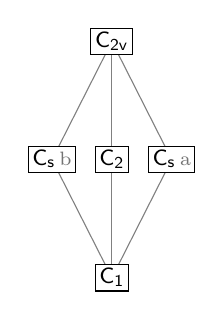
\begin{tikzpicture}[x=1cm, y=1.500cm,
  every node/.style={fill=white, font=\footnotesize, inner xsep=1.5pt, inner ysep=1.2pt, text height=5.6pt, text depth=1.6pt},
  normal/.style={draw, line width=0.4pt}, cover/.style={black!50, line width=0.4pt}]
\draw[cover] (0.00,0) -- (0.00,1);
\draw[cover] (0.00,0) -- (0.76,1);
\draw[cover] (0.00,0) -- (-0.76,1);
\draw[cover] (0.00,1) -- (0.00,2);
\draw[cover] (0.76,1) -- (0.00,2);
\draw[cover] (-0.76,1) -- (0.00,2);
\node[normal] (n00) at (0.00,0) {$\grp{C_{1}}$};
\node[normal] (n01) at (0.00,1) {$\grp{C_{2}}$};
\node[normal] (n02) at (0.76,1) {$\grp{C_{s}}$\clsletter{a}};
\node[normal] (n03) at (-0.76,1) {$\grp{C_{s}}$\clsletter{b}};
\node[normal] (n04) at (0.00,2) {$\grp{C_{2v}}$};
\end{tikzpicture}
\end{center}
{\small\setlength{\fillwidth}{\textwidth}\addtolength{\fillwidth}{-12\tabcolsep}\setlength{\colwidth}{0pt}\cellmax{$\grp{C_{s}}$\clsletter{a} $\samecls$ $\grp{C_{1v}}$ $\samecls$ $\grp{C_{1h}}$}\cellmax{$\grp{C_{s}}$\clsletter{b} $\samecls$ $\grp{C_{1v}}$ $\samecls$ $\grp{C_{1h}}$}\cellmax{$\grp{C_{2v}}$ $\samecls$ $\grp{D_{1h}}$}\cellmax{$\grp{C_{2}}$ $\samecls$ $\grp{D_{1}}$}\cellmax{subgrp}\cellmax{$\grp{C_{1}}$}\addtolength{\fillwidth}{-\colwidth}\setlength{\colwidth}{0pt}\cellmax{order}\cellmax{1}\cellmax{2}\cellmax{4}\addtolength{\fillwidth}{-\colwidth}\setlength{\colwidth}{0pt}\cellmax{conjugates}\cellmax{1}\addtolength{\fillwidth}{-\colwidth}\setlength{\colwidth}{0pt}\cellmax{normal}\cellmax{yes}\addtolength{\fillwidth}{-\colwidth}\setlength{\colwidth}{0pt}\cellmax{$\grp{N}_{\hairsp \grp{C_{2v}}}(\grp{H})$}\cellmax{$\grp{C_{2v}}$}\addtolength{\fillwidth}{-\colwidth}\setlength{\colwidth}{0pt}\cellmax{$\grp{C}_{\hairsp \grp{C_{2v}}}(\grp{H})$}\cellmax{$\grp{C_{2v}}$}\addtolength{\fillwidth}{-\colwidth}\setlength{\colwidth}{0pt}\cellmax{classes}\cellmax{---}\cellmax{all}\cellmax{$\cls{C_{2}}$}\cellmax{$\cls{\sigma_{d}}$}\cellmax{$\cls{\sigma_{v}}$}\fillcap\begin{longtable}{@{}lrrlll>{\RaggedRight\arraybackslash}p{\fillwidth}@{}}\toprule
subgrp & order & conjugates & normal & $\grp{N}_{\hairsp \grp{C_{2v}}}(\grp{H})$ & $\grp{C}_{\hairsp \grp{C_{2v}}}(\grp{H})$ & classes\\\midrule\endhead
\bottomrule\endfoot\endlastfoot
\href{C1.pdf}{$\grp{C_{1}}$} & 1 & 1 & yes & \href{C2v.pdf}{$\grp{C_{2v}}$} & \href{C2v.pdf}{$\grp{C_{2v}}$} & ---\\*
\href{C2.pdf}{$\grp{C_{2}}$} $\samecls$ \href{D1.pdf}{$\grp{D_{1}}$} & 2 & 1 & yes & \href{C2v.pdf}{$\grp{C_{2v}}$} & \href{C2v.pdf}{$\grp{C_{2v}}$} & $\cls{C_{2}}$\\
\href{C1v.pdf}{$\grp{C_{s}}$}\clsletter{a} $\samecls$ \href{C1v.pdf}{$\grp{C_{1v}}$} $\samecls$ \href{C1h.pdf}{$\grp{C_{1h}}$} & 2 & 1 & yes & \href{C2v.pdf}{$\grp{C_{2v}}$} & \href{C2v.pdf}{$\grp{C_{2v}}$} & $\cls{\sigma_{v}}$\\
\href{C1v.pdf}{$\grp{C_{s}}$}\clsletter{b} $\samecls$ \href{C1v.pdf}{$\grp{C_{1v}}$} $\samecls$ \href{C1h.pdf}{$\grp{C_{1h}}$} & 2 & 1 & yes & \href{C2v.pdf}{$\grp{C_{2v}}$} & \href{C2v.pdf}{$\grp{C_{2v}}$} & $\cls{\sigma_{d}}$\\*
\href{C2v.pdf}{$\grp{C_{2v}}$} $\samecls$ \href{D1h.pdf}{$\grp{D_{1h}}$} & 4 & 1 & yes & \href{C2v.pdf}{$\grp{C_{2v}}$} & \href{C2v.pdf}{$\grp{C_{2v}}$} & all\\
\bottomrule\end{longtable}}
\needspace{103pt}
\section{Descent of symmetry}\label{s:subduction}
Conventions: \href{../../CONVENTIONS.pdf}{CONVENTIONS.pdf}, sections \href{../../CONVENTIONS.pdf\#conv.12.2}{12.2} and \href{../../CONVENTIONS.pdf\#conv.12.4}{12.4}.
A column is a class of subgroups $\grp{H}$, in the order of the table of section~\ref{s:subgroups}. The row subgrp names it by its symbol, as in that table, with the letter that distinguishes classes with the same symbol, which are not conjugate in $\grp{C_{2v}}$. The symbol links to the document of $\grp{H}$. The entry of row $\Gamma$ is $\restr{\Gamma}{\grp{H}}$, the restriction of $\Gamma$ along a monomorphism from the record of $\grp{H}$ onto the subgroup, as a sum of the irreps of $\grp{H}$. The monomorphism identifies the subgroup with its record, and $\grp{H}$ names both.
{\small\begin{longtable}{@{}lccc@{}}\toprule
subgrp & \href{C2.pdf}{$\grp{C_{2}}$} & \href{C1v.pdf}{$\grp{C_{s}}$}\clsletter{a} & \href{C1v.pdf}{$\grp{C_{s}}$}\clsletter{b}\\\midrule\endhead
\bottomrule\endfoot\endlastfoot
$\irr{a}_{1}$ & $\irr{a}$ & $\irr{a}'$ & $\irr{a}'$\\*
$\irr{a}_{2}$ & $\irr{a}$ & $\irr{a}''$ & $\irr{a}''$\\*
$\irr{b}_{1}$ & $\irr{b}$ & $\irr{a}'$ & $\irr{a}''$\\*
$\irr{b}_{2}$ & $\irr{b}$ & $\irr{a}''$ & $\irr{a}'$\\
\bottomrule\end{longtable}}
\leavevmode\label{n:irrep.Delta}Read down a column, a table gives induction (Frobenius reciprocity): $\Gamma$ occurs in $\Ind{\grp{H}}{\grp{C_{2v}}} \Lambda$ as often as $\Lambda$ occurs in the entry of row $\Gamma$. For every entry, the record holds the unitary matrix that carries $\restr{\Gamma}{\grp{H}}$ into the direct sum of the matrices of $\grp{H}$ (\texttt{subduction[].blocks}). For every class $\grp{H}$ it holds the left coset representatives (\texttt{transversal}). From both, $\Ind{\grp{H}}{\grp{C_{2v}}} \Lambda$ and its intertwiners follow as in \href{../../CONVENTIONS.pdf}{CONVENTIONS.pdf}, section \href{../../CONVENTIONS.pdf\#conv.12.4}{12.4}.
\needspace{171pt}
\partbox{Permutation representations}
\section{Figures}\label{s:permutation}
Conventions: \href{../../CONVENTIONS.pdf}{CONVENTIONS.pdf}, sections \href{../../CONVENTIONS.pdf\#conv.12.4}{12.4} to \href{../../CONVENTIONS.pdf\#conv.12.6}{12.6}.
Every class of subgroups $\grp{H}$ is the stabilizer of a figure in space, the subgroup of the elements that carry it into itself. \label{n:local.orbit.size}\label{n:element.coset.least}\label{n:index.coset}The group $\grp{C_{2v}}$ permutes the $N = [\grp{C_{2v}} : \grp{H}]$ copies of the figure as it permutes the right cosets $\grp{H}\xi_j$, $j = 0, 1, \dots, N - 1$, ordered by the indices of their least elements $\xi_j$ ($\xi_0 = \cls{E}$). The copy $j$ is the figure moved by $\xi_j$. The matrices $P(g)$ of the defining representation of $\grp{C_{2v}}$ (section~\ref{s:elements}) generate the copies, and the root point $\pointr_0$ of the figure moves to the point $\pointr_j = \pointr_0\, P(\xi_j)$ of the copy $j$. \label{n:local.coset.image}The element $g$ moves the copy $j$ to the copy $j'$, where $\grp{H}\xi_j g = \grp{H}\xi_{j'}$. \label{n:local.matrix.permutation}Its permutation matrix $D(g)$ has the one nonzero entry of row $j$ in column $j'$,
\begin{equation}\label{e:perm.matrix}\pointr_j\, P(g) = \pointr_{j'}, \qquad D(g)_{j,j'} = 1,\end{equation}
and it obeys $D(g)\, D(h) = D(gh)$. The record holds the coordinates of the points of every copy, the images $j'$ of every copy under every element and the table of marks (\href{../../CONVENTIONS.pdf}{CONVENTIONS.pdf}, sections \href{../../CONVENTIONS.pdf\#conv.12.5}{12.5} and \href{../../CONVENTIONS.pdf\#conv.12.6}{12.6}).
\leavevmode\label{n:head.figure}The figure of a class is the first of these whose stabilizer is $\grp{H}$: the point $\pointr_0$, the line through the origin along $\pointr_0$, a spin, a spinning arrow and a helix. Otherwise the figure is the least orbit of $\pointr_0$ under $\grp{H}$ whose stabilizer is $\grp{H}$, a segment, a polygon or a polyhedron. A spin is the axial vector $\pointr_0$, a sense of rotation about its line. A spinning arrow is the arrow $\pointr_0$ with a sense of rotation about itself, and a helix is the line along $\pointr_0$ with a handedness. These two figures are tried only when $\grp{H}$ has no improper element and $\grp{C_{2v}}$ has one. The table lists the classes of subgroups in the order and with the names of the table of section~\ref{s:subgroups}. \label{n:head.site}A row gives $N$, the figure by its shape or number of points, the stabilizer of the point $\pointr_0$ (site), which tells the symmetry elements of $\grp{C_{2v}}$ that the figure lies on, and $\pointr_0$. \label{n:head.vertices}The column vertices gives what the points of all the copies form (the tips of the arrows and spins, both ends of the lines and helices), with ${\times}k$ when $k > 1$ copies pass through each. \label{n:head.rank}The rank counts the classes of pairs of copies under $\grp{C_{2v}}$, including that of a copy with itself. \label{n:head.cos}For a point, line or spin of rank at most 5, the column cos gives the cosine of the angle between two copies (of the acute angle, for lines) for each remaining class of pairs. \label{n:head.hand}The column hand gives 2 when $\grp{H}$ has no improper element and $\grp{C_{2v}}$ has one, so that the rotations of $\grp{C_{2v}}$ leave the copies in two classes, mirror images of each other. These classes are the left- and the right-handed copies of a chiral figure.
{\small\setlength{\tabcolsep}{4pt}\setlength{\fillwidth}{\textwidth}\addtolength{\fillwidth}{-16\tabcolsep}\setlength{\colwidth}{0pt}\cellmax{subgrp}\cellmax{$\grp{C_{2v}}$}\cellmax{$\grp{C_{s}}$\clsletter{a}}\cellmax{$\grp{C_{s}}$\clsletter{b}}\cellmax{$\grp{C_{1}}$}\cellmax{$\grp{C_{2}}$}\addtolength{\fillwidth}{-\colwidth}\setlength{\colwidth}{0pt}\cellmax{$N$}\cellmax{1}\cellmax{2}\cellmax{4}\addtolength{\fillwidth}{-\colwidth}\setlength{\colwidth}{0pt}\cellmax{figure}\cellmax{point}\cellmax{line}\addtolength{\fillwidth}{-\colwidth}\setlength{\colwidth}{0pt}\cellmax{$\grp{C_{2v}}$}\cellmax{$\grp{C_{s}}$\clsletter{a}}\cellmax{$\grp{C_{s}}$\clsletter{b}}\cellmax{site}\cellmax{$\grp{C_{1}}$}\addtolength{\fillwidth}{-\colwidth}\setlength{\colwidth}{0pt}\cellmax{$(0, 0, 1)$}\cellmax{$(0, 1, 2)$}\cellmax{$(1, 0, 2)$}\cellmax{$(1, 2, 0)$}\cellmax{$(1, 2, 4)$}\cellmax{$\pointr_0$}\addtolength{\fillwidth}{-\colwidth}\setlength{\colwidth}{0pt}\cellmax{rectangle}\cellmax{vertices}\cellmax{segment}\cellmax{point}\addtolength{\fillwidth}{-\colwidth}\setlength{\colwidth}{0pt}\cellmax{rank}\cellmax{1}\cellmax{2}\cellmax{4}\addtolength{\fillwidth}{-\colwidth}\setlength{\colwidth}{0pt}\cellmax{hand}\cellmax{2}\cellmax{}\addtolength{\fillwidth}{-\colwidth}\setlength{\colwidth}{0pt}\cellmax{${\tfrac{11}{21}}$, ${\tfrac{13}{21}}$, ${\tfrac{19}{21}}$}\cellmax{cos}\cellmax{${\tfrac{3}{5}}$}\fillcap{\renewcommand{\arraystretch}{1.3}\begin{longtable}{@{}lrllllr>{\RaggedRight\arraybackslash}p{\fillwidth}r@{}}\toprule
subgrp & $N$ & figure & site & $\pointr_0$ & vertices & rank & cos & hand\\\midrule\endhead
\bottomrule\endfoot\endlastfoot
\href{C1.pdf}{$\grp{C_{1}}$} & 4 & point & \href{C1.pdf}{$\grp{C_{1}}$} & $(1, 2, 4)$ & rectangle & 4 & ${\tfrac{11}{21}}$, ${\tfrac{13}{21}}$, ${\tfrac{19}{21}}$ & 2\\*
\href{C2.pdf}{$\grp{C_{2}}$} & 2 & line & \href{C1.pdf}{$\grp{C_{1}}$} & $(1, 2, 0)$ & rectangle & 2 & ${\tfrac{3}{5}}$ & 2\\
\href{C1v.pdf}{$\grp{C_{s}}$}\clsletter{a} & 2 & point & \href{C1v.pdf}{$\grp{C_{s}}$}\clsletter{a} & $(1, 0, 2)$ & segment & 2 & ${\tfrac{3}{5}}$ & \\
\href{C1v.pdf}{$\grp{C_{s}}$}\clsletter{b} & 2 & point & \href{C1v.pdf}{$\grp{C_{s}}$}\clsletter{b} & $(0, 1, 2)$ & segment & 2 & ${\tfrac{3}{5}}$ & \\*
\href{C2v.pdf}{$\grp{C_{2v}}$} & 1 & point & \href{C2v.pdf}{$\grp{C_{2v}}$} & $(0, 0, 1)$ & point & 1 &  & \\
\bottomrule\end{longtable}}}
A uniform polyhedron has regular faces and all its vertices alike. Some points give orbits that are uniform polyhedra or regular polygons: a square for \href{C1.pdf}{$\grp{C_{1}}$}.
\needspace{153pt}
\section{Decompositions}\label{s:decompositions}
Conventions: \href{../../CONVENTIONS.pdf}{CONVENTIONS.pdf}, sections \href{../../CONVENTIONS.pdf\#conv.12.4}{12.4} and \href{../../CONVENTIONS.pdf\#conv.12.5}{12.5}.
The kernel of the permutation representation of a class of subgroups is the subgroup of the elements that leave every copy in place. The decomposition is that of $D$, whose character at $g$ is the number of copies that $g$ leaves in place. An irrep occurs in $D$ as often as the trivial irrep of $\grp{H}$ occurs in its restriction to $\grp{H}$ (section~\ref{s:subduction}).
{\small\medmuskip=4mu plus 2mu\relax\setlength{\fillwidth}{\textwidth}\addtolength{\fillwidth}{-6\tabcolsep}\setlength{\colwidth}{0pt}\cellmax{subgrp}\cellmax{$\grp{C_{2v}}$}\cellmax{$\grp{C_{s}}$\clsletter{a}}\cellmax{$\grp{C_{s}}$\clsletter{b}}\cellmax{$\grp{C_{1}}$}\cellmax{$\grp{C_{2}}$}\addtolength{\fillwidth}{-\colwidth}\setlength{\colwidth}{0pt}\cellmax{$N$}\cellmax{1}\cellmax{2}\cellmax{4}\addtolength{\fillwidth}{-\colwidth}\setlength{\colwidth}{0pt}\cellmax{kernel}\cellmax{$\grp{C_{2v}}$}\cellmax{$\grp{C_{s}}$\clsletter{a}}\cellmax{$\grp{C_{s}}$\clsletter{b}}\cellmax{$\grp{C_{1}}$}\cellmax{$\grp{C_{2}}$}\addtolength{\fillwidth}{-\colwidth}\setlength{\colwidth}{0pt}\cellmax{$\irr{a}_{1}\oplus \irr{a}_{2}\oplus \irr{b}_{1}\oplus \irr{b}_{2}$}\cellmax{decomposition}\cellmax{$\irr{a}_{1}\oplus \irr{a}_{2}$}\cellmax{$\irr{a}_{1}\oplus \irr{b}_{1}$}\cellmax{$\irr{a}_{1}\oplus \irr{b}_{2}$}\cellmax{$\irr{a}_{1}$}\fillcap\begin{longtable}{@{}lrl>{\RaggedRight\arraybackslash}p{\fillwidth}@{}}\toprule
subgrp & $N$ & kernel & decomposition\\\midrule\endhead
\bottomrule\endfoot\endlastfoot
\href{C1.pdf}{$\grp{C_{1}}$} & 4 & \href{C1.pdf}{$\grp{C_{1}}$} & $\irr{a}_{1}\oplus \irr{a}_{2}\oplus \irr{b}_{1}\oplus \irr{b}_{2}$\\*
\href{C2.pdf}{$\grp{C_{2}}$} & 2 & \href{C2.pdf}{$\grp{C_{2}}$} & $\irr{a}_{1}\oplus \irr{a}_{2}$\\
\href{C1v.pdf}{$\grp{C_{s}}$}\clsletter{a} & 2 & \href{C1v.pdf}{$\grp{C_{s}}$}\clsletter{a} & $\irr{a}_{1}\oplus \irr{b}_{1}$\\
\href{C1v.pdf}{$\grp{C_{s}}$}\clsletter{b} & 2 & \href{C1v.pdf}{$\grp{C_{s}}$}\clsletter{b} & $\irr{a}_{1}\oplus \irr{b}_{2}$\\*
\href{C2v.pdf}{$\grp{C_{2v}}$} & 1 & \href{C2v.pdf}{$\grp{C_{2v}}$} & $\irr{a}_{1}$\\
\bottomrule\end{longtable}}
\needspace{103pt}
\section{Cycle types}\label{s:cycle_types}
Conventions: \href{../../CONVENTIONS.pdf}{CONVENTIONS.pdf}, section \href{../../CONVENTIONS.pdf\#conv.12.5}{12.5}.
\leavevmode\label{n:local.cycle.type}\label{n:local.cycle.length}\label{n:local.cycle.count}The entry in the row of a class of subgroups and the column of a class of elements is the cycle type of $j \mapsto j'$ for these elements, written $\ell^{c}$ for $c$ cycles of length $\ell$. The cycles of length 1 are the copies that the element leaves in place, whose number is the character of $D$. \label{n:local.cycles}\label{n:local.states}With $c(g)$ cycles in all, $g$ has the character $q^{c(g)}$ on the $q^N$ products of one of $q$ states of each copy (\href{../../CONVENTIONS.pdf}{CONVENTIONS.pdf}, section \href{../../CONVENTIONS.pdf\#conv.12.5}{12.5}).
{\small\setlength{\tabcolsep}{4pt}\begin{longtable}{@{}lrcccc@{}}\toprule
subgrp & $N$ & $\cls{E}$ & $\cls{C_{2}}$ & $\cls{\sigma_{v}}$ & $\cls{\sigma_{d}}$\\\midrule\endhead
\bottomrule\endfoot\endlastfoot
\href{C1.pdf}{$\grp{C_{1}}$} & 4 & $1^{4}$ & $2^{2}$ & $2^{2}$ & $2^{2}$\\*
\href{C2.pdf}{$\grp{C_{2}}$} & 2 & $1^{2}$ & $1^{2}$ & $2$ & $2$\\*
\href{C1v.pdf}{$\grp{C_{s}}$}\clsletter{a} & 2 & $1^{2}$ & $2$ & $1^{2}$ & $2$\\*
\href{C1v.pdf}{$\grp{C_{s}}$}\clsletter{b} & 2 & $1^{2}$ & $2$ & $2$ & $1^{2}$\\
\bottomrule\end{longtable}}
\needspace{177pt}
\partbox{Angular momentum}
\section{Subduction from \texorpdfstring{$\grp{O(3)}$}{O(3)}}\label{s:subduction_o3}
Conventions: \href{../../CONVENTIONS.pdf}{CONVENTIONS.pdf}, sections \href{../../CONVENTIONS.pdf\#conv.11}{11} and \href{../../CONVENTIONS.pdf\#conv.14.1}{14.1}.
\leavevmode\label{n:index.J}\label{n:index.parity}\label{n:function.multiplicity}The irrep $\irrJp{J}{p}$ of \href{O3.pdf}{$\grp{O(3)}$} has angular momentum $J$ and parity $p$ ($\ptag{g}$ for $p = +1$, $\ptag{u}$ for $p = -1$), and $b_\Gamma(J, p)$ is the multiplicity of $\Gamma$ in
\begin{equation}\label{e:o3}\restr{\irrJp{J}{p}}{\grp{C_{2v}}} .\end{equation}
\leavevmode\label{n:index.increment}Each table gives $b_\Gamma(J, p)$ for $J \le 20$, and $b_\Gamma(J + 2, p) = b_\Gamma(J, p) + \Delta_\Gamma$ for every $J$, where $\Delta_\Gamma$ is the last row of the table of parity $p$.
The determinant exchanges the parities: $\irrJp{J}{-1} = \irrJp{J}{+1} \irrprod \det$, so that $b_\Gamma(J, -1) = b_{\Gamma \irrprod \det_{\grp{C_{2v}}}}(J, +1)$.
\needspace{182pt}
\paragraph{Parity $\ptag{g}$ ($p = +1$).}
{\small\begin{longtable}{@{}rrrrr@{\hspace{18pt}}rrrrr@{\hspace{18pt}}rrrrr@{}}\toprule
$J$ & $\irr{a}_{1}$ & $\irr{a}_{2}$ & $\irr{b}_{1}$ & $\irr{b}_{2}$ & $J$ & $\irr{a}_{1}$ & $\irr{a}_{2}$ & $\irr{b}_{1}$ & $\irr{b}_{2}$ & $J$ & $\irr{a}_{1}$ & $\irr{a}_{2}$ & $\irr{b}_{1}$ & $\irr{b}_{2}$\\\midrule\endhead
\bottomrule\endfoot\endlastfoot
0 & 1 & 0 & 0 & 0 & 8 & 5 & 4 & 4 & 4 & 16 & 9 & 8 & 8 & 8\\*
1 & 0 & 1 & 1 & 1 & 9 & 4 & 5 & 5 & 5 & 17 & 8 & 9 & 9 & 9\\*
2 & 2 & 1 & 1 & 1 & 10 & 6 & 5 & 5 & 5 & 18 & 10 & 9 & 9 & 9\\*
3 & 1 & 2 & 2 & 2 & 11 & 5 & 6 & 6 & 6 & 19 & 9 & 10 & 10 & 10\\*
4 & 3 & 2 & 2 & 2 & 12 & 7 & 6 & 6 & 6 & 20 & 11 & 10 & 10 & 10\\*\noalign{\vskip 1.5pt}\multispan{5} & \multispan{5} & \multispan{5}\leaders\hrule height\cmidrulewidth\hfill\kern0pt\\*\noalign{\vskip 1.5pt}
5 & 2 & 3 & 3 & 3 & 13 & 6 & 7 & 7 & 7 & $\Delta_\Gamma$ & 1 & 1 & 1 & 1\\*
6 & 4 & 3 & 3 & 3 & 14 & 8 & 7 & 7 & 7 &  &  &  &  & \\*
7 & 3 & 4 & 4 & 4 & 15 & 7 & 8 & 8 & 8 &  &  &  &  & \\
\bottomrule\end{longtable}}
\needspace{182pt}
\paragraph{Parity $\ptag{u}$ ($p = -1$).}
{\small\begin{longtable}{@{}rrrrr@{\hspace{18pt}}rrrrr@{\hspace{18pt}}rrrrr@{}}\toprule
$J$ & $\irr{a}_{1}$ & $\irr{a}_{2}$ & $\irr{b}_{1}$ & $\irr{b}_{2}$ & $J$ & $\irr{a}_{1}$ & $\irr{a}_{2}$ & $\irr{b}_{1}$ & $\irr{b}_{2}$ & $J$ & $\irr{a}_{1}$ & $\irr{a}_{2}$ & $\irr{b}_{1}$ & $\irr{b}_{2}$\\\midrule\endhead
\bottomrule\endfoot\endlastfoot
0 & 0 & 1 & 0 & 0 & 8 & 4 & 5 & 4 & 4 & 16 & 8 & 9 & 8 & 8\\*
1 & 1 & 0 & 1 & 1 & 9 & 5 & 4 & 5 & 5 & 17 & 9 & 8 & 9 & 9\\*
2 & 1 & 2 & 1 & 1 & 10 & 5 & 6 & 5 & 5 & 18 & 9 & 10 & 9 & 9\\*
3 & 2 & 1 & 2 & 2 & 11 & 6 & 5 & 6 & 6 & 19 & 10 & 9 & 10 & 10\\*
4 & 2 & 3 & 2 & 2 & 12 & 6 & 7 & 6 & 6 & 20 & 10 & 11 & 10 & 10\\*\noalign{\vskip 1.5pt}\multispan{5} & \multispan{5} & \multispan{5}\leaders\hrule height\cmidrulewidth\hfill\kern0pt\\*\noalign{\vskip 1.5pt}
5 & 3 & 2 & 3 & 3 & 13 & 7 & 6 & 7 & 7 & $\Delta_\Gamma$ & 1 & 1 & 1 & 1\\*
6 & 3 & 4 & 3 & 3 & 14 & 7 & 8 & 7 & 7 &  &  &  &  & \\*
7 & 4 & 3 & 4 & 4 & 15 & 8 & 7 & 8 & 8 &  &  &  &  & \\
\bottomrule\end{longtable}}
\needspace{110pt}
\section{Multiplicities and allowed \texorpdfstring{$m$}{m}}\label{s:multiplicities}
Conventions: \href{../../CONVENTIONS.pdf}{CONVENTIONS.pdf}, section \href{../../CONVENTIONS.pdf\#conv.14}{14}.
\leavevmode\label{n:function.generating}\label{n:index.generating.variable}\label{n:function.generating.numerator}The multiplicity $b_\Gamma(J) = b_\Gamma(J, (-1)^J)$ is the number of blocks of $\Gamma$ at $J$, with the generating function
\begin{equation}\label{e:gf}H_\Gamma(t) = \sum_{J\ge0} b_\Gamma(J)\,t^J = P_\Gamma(t)/((1-t)(1-t^{2})).\end{equation}
\leavevmode\label{n:delimiter.floor}\label{n:local.floor.x}\label{n:function.count}\label{n:index.modulus.K}\label{n:index.residue}The closed forms of $b_\Gamma(J)$ use the floor $\lfloor x\rfloor$, the greatest integer $\le x$, and
\begin{equation}\label{e:count}n_K(J,q) = \Bigl\lfloor\frac{J-q}{K}\Bigr\rfloor + \Bigl\lfloor\frac{J+q}{K}\Bigr\rfloor + 1 = \#\{m\in[-J,J] : m\equiv q \pmod{K}\}.\end{equation}
\leavevmode\label{n:head.parity}The listed residues are the $m \bmod 2$ of the nonzero components of the vectors of $\Gamma$. A dash means no block of $\Gamma$ at that parity of $J$.
{\small{\renewcommand{\arraystretch}{1.3}\begin{longtable}{@{}llllll@{}}\toprule
$\Gamma$ & $P_\Gamma(t)$ & $b_\Gamma(J)$, $J$ even & $J$ odd & $m \bmod 2$, $J$ even & $J$ odd\\\midrule\endhead
\bottomrule\endfoot\endlastfoot
$\irr{a}_{1}$ & $1$ & $\bigl\lfloor\tfrac{J}{2}\bigr\rfloor + 1$ & $\bigl\lfloor\tfrac{J}{2}\bigr\rfloor + 1$ & 0 & 0\\*
$\irr{a}_{2}$ & $t^{2}$ & $\bigl\lfloor\tfrac{J}{2}\bigr\rfloor$ & $\bigl\lfloor\tfrac{J}{2}\bigr\rfloor$ & 0 & 0\\*
$\irr{b}_{1}$ & $t$ & $\bigl\lfloor\tfrac{J+1}{2}\bigr\rfloor$ & $\bigl\lfloor\tfrac{J+1}{2}\bigr\rfloor$ & 1 & 1\\*
$\irr{b}_{2}$ & $t$ & $\bigl\lfloor\tfrac{J+1}{2}\bigr\rfloor$ & $\bigl\lfloor\tfrac{J+1}{2}\bigr\rfloor$ & 1 & 1\\
\bottomrule\end{longtable}}}
\needspace{110pt}
\section{Symmetry-adapted bases}\label{s:bases}
Conventions: \href{../../CONVENTIONS.pdf}{CONVENTIONS.pdf}, section \href{../../CONVENTIONS.pdf\#conv.14.1}{14.1}.
The constant $\iunit$ is the imaginary unit.
\leavevmode\label{n:index.m}\label{n:vector.ket}The kets $\jm{J}{m}$ are the spherical harmonics (the inversion acts as $(-1)^J$). \label{n:index.ketcoefficient}\label{n:vector.basis.symmetry}\label{n:index.ketweight}\label{n:index.total}A vector is listed by its coefficients $e_m$:
\begin{equation}\label{e:ket}v = \frac{1}{\sqrt{\mathrm{tot}}}\sum_m e_m\sqrt{F_m}\;\jm{J}{m},\qquad F_m = (J+m)!\,(J-m)!,\qquad \mathrm{tot} = \sum_m |e_m|^2F_m,\end{equation}
\leavevmode\label{n:index.pair.sign}so a single ket has amplitude 1, and a pair $\jm{J}{m} + s\,\jm{J}{-m}$, $s = \pm1$, has amplitudes $\tfrac{1}{2}\sqrt{2}$ and $\tfrac{1}{2}s\sqrt{2}$, or these times $\iunit$. Each $e_m$ is $\pm1$ or $\pm\iunit$.
\leavevmode\label{n:group.A}\label{n:function.character.abelian}The subgroup $\grp{A} = \grp{C_{2v}}\cap\grp{C_{\infty h}}$ acts diagonally on the kets, on $\jm{J}{m}$ by the character $\chiA(m)$, and $\grpindex{\grp{C_{2v}}}{\grp{A}} = 2$. \label{n:element.mirror.angle}The flip $\elt{\sigma_v}(0)$, the mirror in the $xz$ plane, sends $m$ to $-m$. Every irrep is one-dimensional, so a block is one ket or a pair. Kets $\jm{J}{m}$ and $\jm{J}{-m}$ of one character of $\grp{A}$ give two one-dimensional blocks $\jm{J}{m} + s\,\jm{J}{-m}$, $s = \pm1$, the one with $s = -(-1)^m$ times $\iunit$. The factor $\iunit$ makes each block adapted to time reversal (\href{../../CONVENTIONS.pdf}{CONVENTIONS.pdf}, section \href{../../CONVENTIONS.pdf\#conv.14}{14}). Blocks are ordered by $J$, then $|m|$, a pair with $s = +1$ first (\href{../../CONVENTIONS.pdf}{CONVENTIONS.pdf}, section \href{../../CONVENTIONS.pdf\#conv.14.1}{14.1}).
\leavevmode\label{n:head.case}\label{n:head.partners}The table lists every case of block, its dimension $d$ and its partners in order.
\begin{center}\begin{tabular}{@{}lrl@{}}\toprule
case & $d$ & partners\\\midrule
$\chiA(m) = \chiA(-m)$, $m > 0$, $s = (-1)^m$ & 1 & $\jm{J}{m} + s\,\jm{J}{-m}$\\
$\chiA(m) = \chiA(-m)$, $m > 0$, $s = -(-1)^m$ & 1 & $\iunit(\jm{J}{m} + s\,\jm{J}{-m})$\\
$m = 0$ & 1 & $\jm{J}{0}$\\
\bottomrule\end{tabular}\end{center}
The bases have 121 blocks and 121 vectors at $J = 0, 1, \dots, 10$. \label{n:index.copy}\label{n:head.vector}A row gives a vector of a block at $J$: the block's irrep and copy index $\mult$, the partner index $\intx$ and the vector.
{\small\setlength{\tabcolsep}{3pt}\begin{longtable}{@{}rlrr@{\hspace{4pt}}l@{\hspace{18pt}}rlrr@{\hspace{4pt}}l@{}}\toprule
$J$ & irrep & $\mult$ & $\intx$ & vector & $J$ & irrep & $\mult$ & $\intx$ & vector\\\midrule\endhead
\bottomrule\endfoot\endlastfoot
0 & $\irr{a}_{1}$ & 1 & 1 & $\jm{0}{0}$ & 3 & $\irr{b}_{1}$ & 1 & 1 & $\jm{3}{1}$ $-\jm{3}{-1}$\\*\noalign{\vskip 1.5pt}\multispan{5}\leaders\hrule height\cmidrulewidth\hfill\kern0pt\hskip18pt & \multispan{5}\\*\noalign{\vskip 1.5pt}
1 & $\irr{a}_{1}$ & 1 & 1 & $\jm{1}{0}$ & 3 & $\irr{a}_{1}$ & 2 & 1 & $\jm{3}{2}$ $+$ $\jm{3}{-2}$\\*
1 & $\irr{b}_{2}$ & 1 & 1 & $\iunit{}\,\jm{1}{1}$ $+$ $\iunit{}\,\jm{1}{-1}$ & 3 & $\irr{a}_{2}$ & 1 & 1 & $\iunit{}\,\jm{3}{2}$ $-\iunit{}\,\jm{3}{-2}$\\*
1 & $\irr{b}_{1}$ & 1 & 1 & $\jm{1}{1}$ $-\jm{1}{-1}$ & 3 & $\irr{b}_{2}$ & 2 & 1 & $\iunit{}\,\jm{3}{3}$ $+$ $\iunit{}\,\jm{3}{-3}$\\*\noalign{\vskip 1.5pt}\multispan{5}\leaders\hrule height\cmidrulewidth\hfill\kern0pt\hskip18pt & \multispan{5}\\*\noalign{\vskip 1.5pt}
2 & $\irr{a}_{1}$ & 1 & 1 & $\jm{2}{0}$ & 3 & $\irr{b}_{1}$ & 2 & 1 & $\jm{3}{3}$ $-\jm{3}{-3}$\\*\noalign{\vskip 1.5pt}\multispan{5} & \multispan{5}\leaders\hrule height\cmidrulewidth\hfill\kern0pt\\*\noalign{\vskip 1.5pt}
2 & $\irr{b}_{2}$ & 1 & 1 & $\iunit{}\,\jm{2}{1}$ $+$ $\iunit{}\,\jm{2}{-1}$ & 4 & $\irr{a}_{1}$ & 1 & 1 & $\jm{4}{0}$\\*
2 & $\irr{b}_{1}$ & 1 & 1 & $\jm{2}{1}$ $-\jm{2}{-1}$ & 4 & $\irr{b}_{2}$ & 1 & 1 & $\iunit{}\,\jm{4}{1}$ $+$ $\iunit{}\,\jm{4}{-1}$\\*
2 & $\irr{a}_{1}$ & 2 & 1 & $\jm{2}{2}$ $+$ $\jm{2}{-2}$ & 4 & $\irr{b}_{1}$ & 1 & 1 & $\jm{4}{1}$ $-\jm{4}{-1}$\\*
2 & $\irr{a}_{2}$ & 1 & 1 & $\iunit{}\,\jm{2}{2}$ $-\iunit{}\,\jm{2}{-2}$ & 4 & $\irr{a}_{1}$ & 2 & 1 & $\jm{4}{2}$ $+$ $\jm{4}{-2}$\\*\noalign{\vskip 1.5pt}\multispan{5}\leaders\hrule height\cmidrulewidth\hfill\kern0pt\hskip18pt & \multispan{5}\\*\noalign{\vskip 1.5pt}
3 & $\irr{a}_{1}$ & 1 & 1 & $\jm{3}{0}$ & 4 & $\irr{a}_{2}$ & 1 & 1 & $\iunit{}\,\jm{4}{2}$ $-\iunit{}\,\jm{4}{-2}$\\*
3 & $\irr{b}_{2}$ & 1 & 1 & $\iunit{}\,\jm{3}{1}$ $+$ $\iunit{}\,\jm{3}{-1}$ & 4 & $\irr{b}_{2}$ & 2 & 1 & $\iunit{}\,\jm{4}{3}$ $+$ $\iunit{}\,\jm{4}{-3}$\\
\grouprule{0pt}{\heavyrulewidth}
4 & $\irr{b}_{1}$ & 2 & 1 & $\jm{4}{3}$ $-\jm{4}{-3}$ & 5 & $\irr{a}_{2}$ & 2 & 1 & $\iunit{}\,\jm{5}{4}$ $-\iunit{}\,\jm{5}{-4}$\\*
4 & $\irr{a}_{1}$ & 3 & 1 & $\jm{4}{4}$ $+$ $\jm{4}{-4}$ & 5 & $\irr{b}_{2}$ & 3 & 1 & $\iunit{}\,\jm{5}{5}$ $+$ $\iunit{}\,\jm{5}{-5}$\\*
4 & $\irr{a}_{2}$ & 2 & 1 & $\iunit{}\,\jm{4}{4}$ $-\iunit{}\,\jm{4}{-4}$ & 5 & $\irr{b}_{1}$ & 3 & 1 & $\jm{5}{5}$ $-\jm{5}{-5}$\\*\noalign{\vskip 1.5pt}\multispan{5}\leaders\hrule height\cmidrulewidth\hfill\kern0pt\hskip18pt & \multispan{5}\leaders\hrule height\cmidrulewidth\hfill\kern0pt\\*\noalign{\vskip 1.5pt}
5 & $\irr{a}_{1}$ & 1 & 1 & $\jm{5}{0}$ & 6 & $\irr{a}_{1}$ & 1 & 1 & $\jm{6}{0}$\\*
5 & $\irr{b}_{2}$ & 1 & 1 & $\iunit{}\,\jm{5}{1}$ $+$ $\iunit{}\,\jm{5}{-1}$ & 6 & $\irr{b}_{2}$ & 1 & 1 & $\iunit{}\,\jm{6}{1}$ $+$ $\iunit{}\,\jm{6}{-1}$\\*
5 & $\irr{b}_{1}$ & 1 & 1 & $\jm{5}{1}$ $-\jm{5}{-1}$ & 6 & $\irr{b}_{1}$ & 1 & 1 & $\jm{6}{1}$ $-\jm{6}{-1}$\\*
5 & $\irr{a}_{1}$ & 2 & 1 & $\jm{5}{2}$ $+$ $\jm{5}{-2}$ & 6 & $\irr{a}_{1}$ & 2 & 1 & $\jm{6}{2}$ $+$ $\jm{6}{-2}$\\*
5 & $\irr{a}_{2}$ & 1 & 1 & $\iunit{}\,\jm{5}{2}$ $-\iunit{}\,\jm{5}{-2}$ & 6 & $\irr{a}_{2}$ & 1 & 1 & $\iunit{}\,\jm{6}{2}$ $-\iunit{}\,\jm{6}{-2}$\\*
5 & $\irr{b}_{2}$ & 2 & 1 & $\iunit{}\,\jm{5}{3}$ $+$ $\iunit{}\,\jm{5}{-3}$ & 6 & $\irr{b}_{2}$ & 2 & 1 & $\iunit{}\,\jm{6}{3}$ $+$ $\iunit{}\,\jm{6}{-3}$\\*
5 & $\irr{b}_{1}$ & 2 & 1 & $\jm{5}{3}$ $-\jm{5}{-3}$ & 6 & $\irr{b}_{1}$ & 2 & 1 & $\jm{6}{3}$ $-\jm{6}{-3}$\\*
5 & $\irr{a}_{1}$ & 3 & 1 & $\jm{5}{4}$ $+$ $\jm{5}{-4}$ & 6 & $\irr{a}_{1}$ & 3 & 1 & $\jm{6}{4}$ $+$ $\jm{6}{-4}$\\
\grouprule{0pt}{\heavyrulewidth}
6 & $\irr{a}_{2}$ & 2 & 1 & $\iunit{}\,\jm{6}{4}$ $-\iunit{}\,\jm{6}{-4}$ & 7 & $\irr{b}_{1}$ & 2 & 1 & $\jm{7}{3}$ $-\jm{7}{-3}$\\*
6 & $\irr{b}_{2}$ & 3 & 1 & $\iunit{}\,\jm{6}{5}$ $+$ $\iunit{}\,\jm{6}{-5}$ & 7 & $\irr{a}_{1}$ & 3 & 1 & $\jm{7}{4}$ $+$ $\jm{7}{-4}$\\*
6 & $\irr{b}_{1}$ & 3 & 1 & $\jm{6}{5}$ $-\jm{6}{-5}$ & 7 & $\irr{a}_{2}$ & 2 & 1 & $\iunit{}\,\jm{7}{4}$ $-\iunit{}\,\jm{7}{-4}$\\*
6 & $\irr{a}_{1}$ & 4 & 1 & $\jm{6}{6}$ $+$ $\jm{6}{-6}$ & 7 & $\irr{b}_{2}$ & 3 & 1 & $\iunit{}\,\jm{7}{5}$ $+$ $\iunit{}\,\jm{7}{-5}$\\*
6 & $\irr{a}_{2}$ & 3 & 1 & $\iunit{}\,\jm{6}{6}$ $-\iunit{}\,\jm{6}{-6}$ & 7 & $\irr{b}_{1}$ & 3 & 1 & $\jm{7}{5}$ $-\jm{7}{-5}$\\*\noalign{\vskip 1.5pt}\multispan{5}\leaders\hrule height\cmidrulewidth\hfill\kern0pt\hskip18pt & \multispan{5}\\*\noalign{\vskip 1.5pt}
7 & $\irr{a}_{1}$ & 1 & 1 & $\jm{7}{0}$ & 7 & $\irr{a}_{1}$ & 4 & 1 & $\jm{7}{6}$ $+$ $\jm{7}{-6}$\\*
7 & $\irr{b}_{2}$ & 1 & 1 & $\iunit{}\,\jm{7}{1}$ $+$ $\iunit{}\,\jm{7}{-1}$ & 7 & $\irr{a}_{2}$ & 3 & 1 & $\iunit{}\,\jm{7}{6}$ $-\iunit{}\,\jm{7}{-6}$\\*
7 & $\irr{b}_{1}$ & 1 & 1 & $\jm{7}{1}$ $-\jm{7}{-1}$ & 7 & $\irr{b}_{2}$ & 4 & 1 & $\iunit{}\,\jm{7}{7}$ $+$ $\iunit{}\,\jm{7}{-7}$\\*
7 & $\irr{a}_{1}$ & 2 & 1 & $\jm{7}{2}$ $+$ $\jm{7}{-2}$ & 7 & $\irr{b}_{1}$ & 4 & 1 & $\jm{7}{7}$ $-\jm{7}{-7}$\\*\noalign{\vskip 1.5pt}\multispan{5} & \multispan{5}\leaders\hrule height\cmidrulewidth\hfill\kern0pt\\*\noalign{\vskip 1.5pt}
7 & $\irr{a}_{2}$ & 1 & 1 & $\iunit{}\,\jm{7}{2}$ $-\iunit{}\,\jm{7}{-2}$ & 8 & $\irr{a}_{1}$ & 1 & 1 & $\jm{8}{0}$\\*
7 & $\irr{b}_{2}$ & 2 & 1 & $\iunit{}\,\jm{7}{3}$ $+$ $\iunit{}\,\jm{7}{-3}$ & 8 & $\irr{b}_{2}$ & 1 & 1 & $\iunit{}\,\jm{8}{1}$ $+$ $\iunit{}\,\jm{8}{-1}$\\
\grouprule{0pt}{\heavyrulewidth}
8 & $\irr{b}_{1}$ & 1 & 1 & $\jm{8}{1}$ $-\jm{8}{-1}$ & 8 & $\irr{b}_{2}$ & 4 & 1 & $\iunit{}\,\jm{8}{7}$ $+$ $\iunit{}\,\jm{8}{-7}$\\*
8 & $\irr{a}_{1}$ & 2 & 1 & $\jm{8}{2}$ $+$ $\jm{8}{-2}$ & 8 & $\irr{b}_{1}$ & 4 & 1 & $\jm{8}{7}$ $-\jm{8}{-7}$\\*
8 & $\irr{a}_{2}$ & 1 & 1 & $\iunit{}\,\jm{8}{2}$ $-\iunit{}\,\jm{8}{-2}$ & 8 & $\irr{a}_{1}$ & 5 & 1 & $\jm{8}{8}$ $+$ $\jm{8}{-8}$\\*
8 & $\irr{b}_{2}$ & 2 & 1 & $\iunit{}\,\jm{8}{3}$ $+$ $\iunit{}\,\jm{8}{-3}$ & 8 & $\irr{a}_{2}$ & 4 & 1 & $\iunit{}\,\jm{8}{8}$ $-\iunit{}\,\jm{8}{-8}$\\*\noalign{\vskip 1.5pt}\multispan{5} & \multispan{5}\leaders\hrule height\cmidrulewidth\hfill\kern0pt\\*\noalign{\vskip 1.5pt}
8 & $\irr{b}_{1}$ & 2 & 1 & $\jm{8}{3}$ $-\jm{8}{-3}$ & 9 & $\irr{a}_{1}$ & 1 & 1 & $\jm{9}{0}$\\*
8 & $\irr{a}_{1}$ & 3 & 1 & $\jm{8}{4}$ $+$ $\jm{8}{-4}$ & 9 & $\irr{b}_{2}$ & 1 & 1 & $\iunit{}\,\jm{9}{1}$ $+$ $\iunit{}\,\jm{9}{-1}$\\*
8 & $\irr{a}_{2}$ & 2 & 1 & $\iunit{}\,\jm{8}{4}$ $-\iunit{}\,\jm{8}{-4}$ & 9 & $\irr{b}_{1}$ & 1 & 1 & $\jm{9}{1}$ $-\jm{9}{-1}$\\*
8 & $\irr{b}_{2}$ & 3 & 1 & $\iunit{}\,\jm{8}{5}$ $+$ $\iunit{}\,\jm{8}{-5}$ & 9 & $\irr{a}_{1}$ & 2 & 1 & $\jm{9}{2}$ $+$ $\jm{9}{-2}$\\*
8 & $\irr{b}_{1}$ & 3 & 1 & $\jm{8}{5}$ $-\jm{8}{-5}$ & 9 & $\irr{a}_{2}$ & 1 & 1 & $\iunit{}\,\jm{9}{2}$ $-\iunit{}\,\jm{9}{-2}$\\*
8 & $\irr{a}_{1}$ & 4 & 1 & $\jm{8}{6}$ $+$ $\jm{8}{-6}$ & 9 & $\irr{b}_{2}$ & 2 & 1 & $\iunit{}\,\jm{9}{3}$ $+$ $\iunit{}\,\jm{9}{-3}$\\*
8 & $\irr{a}_{2}$ & 3 & 1 & $\iunit{}\,\jm{8}{6}$ $-\iunit{}\,\jm{8}{-6}$ & 9 & $\irr{b}_{1}$ & 2 & 1 & $\jm{9}{3}$ $-\jm{9}{-3}$\\
\grouprule{0pt}{\heavyrulewidth}
9 & $\irr{a}_{1}$ & 3 & 1 & $\jm{9}{4}$ $+$ $\jm{9}{-4}$ & 9 & $\irr{b}_{1}$ & 5 & 1 & $\jm{9}{9}$ $-\jm{9}{-9}$\\*\noalign{\vskip 1.5pt}\multispan{5} & \multispan{5}\leaders\hrule height\cmidrulewidth\hfill\kern0pt\\*\noalign{\vskip 1.5pt}
9 & $\irr{a}_{2}$ & 2 & 1 & $\iunit{}\,\jm{9}{4}$ $-\iunit{}\,\jm{9}{-4}$ & 10 & $\irr{a}_{1}$ & 1 & 1 & $\jm{10}{0}$\\*
9 & $\irr{b}_{2}$ & 3 & 1 & $\iunit{}\,\jm{9}{5}$ $+$ $\iunit{}\,\jm{9}{-5}$ & 10 & $\irr{b}_{2}$ & 1 & 1 & $\iunit{}\,\jm{10}{1}$ $+$ $\iunit{}\,\jm{10}{-1}$\\*
9 & $\irr{b}_{1}$ & 3 & 1 & $\jm{9}{5}$ $-\jm{9}{-5}$ & 10 & $\irr{b}_{1}$ & 1 & 1 & $\jm{10}{1}$ $-\jm{10}{-1}$\\*
9 & $\irr{a}_{1}$ & 4 & 1 & $\jm{9}{6}$ $+$ $\jm{9}{-6}$ & 10 & $\irr{a}_{1}$ & 2 & 1 & $\jm{10}{2}$ $+$ $\jm{10}{-2}$\\*
9 & $\irr{a}_{2}$ & 3 & 1 & $\iunit{}\,\jm{9}{6}$ $-\iunit{}\,\jm{9}{-6}$ & 10 & $\irr{a}_{2}$ & 1 & 1 & $\iunit{}\,\jm{10}{2}$ $-\iunit{}\,\jm{10}{-2}$\\*
9 & $\irr{b}_{2}$ & 4 & 1 & $\iunit{}\,\jm{9}{7}$ $+$ $\iunit{}\,\jm{9}{-7}$ & 10 & $\irr{b}_{2}$ & 2 & 1 & $\iunit{}\,\jm{10}{3}$ $+$ $\iunit{}\,\jm{10}{-3}$\\*
9 & $\irr{b}_{1}$ & 4 & 1 & $\jm{9}{7}$ $-\jm{9}{-7}$ & 10 & $\irr{b}_{1}$ & 2 & 1 & $\jm{10}{3}$ $-\jm{10}{-3}$\\*
9 & $\irr{a}_{1}$ & 5 & 1 & $\jm{9}{8}$ $+$ $\jm{9}{-8}$ & 10 & $\irr{a}_{1}$ & 3 & 1 & $\jm{10}{4}$ $+$ $\jm{10}{-4}$\\*
9 & $\irr{a}_{2}$ & 4 & 1 & $\iunit{}\,\jm{9}{8}$ $-\iunit{}\,\jm{9}{-8}$ & 10 & $\irr{a}_{2}$ & 2 & 1 & $\iunit{}\,\jm{10}{4}$ $-\iunit{}\,\jm{10}{-4}$\\*
9 & $\irr{b}_{2}$ & 5 & 1 & $\iunit{}\,\jm{9}{9}$ $+$ $\iunit{}\,\jm{9}{-9}$ & 10 & $\irr{b}_{2}$ & 3 & 1 & $\iunit{}\,\jm{10}{5}$ $+$ $\iunit{}\,\jm{10}{-5}$\\
\grouprule{0pt}{\heavyrulewidth}
10 & $\irr{b}_{1}$ & 3 & 1 & $\jm{10}{5}$ $-\jm{10}{-5}$ & 10 & $\irr{a}_{2}$ & 4 & 1 & $\iunit{}\,\jm{10}{8}$ $-\iunit{}\,\jm{10}{-8}$\\*
10 & $\irr{a}_{1}$ & 4 & 1 & $\jm{10}{6}$ $+$ $\jm{10}{-6}$ & 10 & $\irr{b}_{2}$ & 5 & 1 & $\iunit{}\,\jm{10}{9}$ $+$ $\iunit{}\,\jm{10}{-9}$\\*
10 & $\irr{a}_{2}$ & 3 & 1 & $\iunit{}\,\jm{10}{6}$ $-\iunit{}\,\jm{10}{-6}$ & 10 & $\irr{b}_{1}$ & 5 & 1 & $\jm{10}{9}$ $-\jm{10}{-9}$\\*
10 & $\irr{b}_{2}$ & 4 & 1 & $\iunit{}\,\jm{10}{7}$ $+$ $\iunit{}\,\jm{10}{-7}$ & 10 & $\irr{a}_{1}$ & 6 & 1 & $\jm{10}{10}$ $+$ $\jm{10}{-10}$\\*
10 & $\irr{b}_{1}$ & 4 & 1 & $\jm{10}{7}$ $-\jm{10}{-7}$ & 10 & $\irr{a}_{2}$ & 5 & 1 & $\iunit{}\,\jm{10}{10}$ $-\iunit{}\,\jm{10}{-10}$\\*
10 & $\irr{a}_{1}$ & 5 & 1 & $\jm{10}{8}$ $+$ $\jm{10}{-8}$ &  &  &  &  & \\
\bottomrule\end{longtable}}
\needspace{323pt}
\partbox{Tensors}
\section{\texorpdfstring{$\orbital{s}$, $\orbital{p}$, $\orbital{d}$, $\orbital{f}$}{s, p, d, f} functions}\label{s:orbitals}
Conventions: \href{../../CONVENTIONS.pdf}{CONVENTIONS.pdf}, section \href{../../CONVENTIONS.pdf\#conv.13}{13}.
\leavevmode\label{n:head.function}A function is a real solid harmonic $\orbital{s}$, $\orbital{p}$, $\orbital{d}$ or $\orbital{f}$, of degree 0 to 3 with coprime integer coefficients, or a component $\orbital{R}_{x}$, $\orbital{R}_{y}$, $\orbital{R}_{z}$ of an axial vector. \label{n:head.polynomial}\label{n:head.irreps}A row gives the function, its polynomial in $x$, $y$ and $z$, and the irreps of its nonzero isotypic components.
{\small\begin{longtable}{@{}lll@{\hspace{18pt}}lll@{}}\toprule
function & polynomial & irreps & function & polynomial & irreps\\\midrule\endhead
\bottomrule\endfoot\endlastfoot
$\orbital{s}$ & $1$ & $\irr{a}_{1}$ & $\orbital{f}_{xz^2}$ & $-x^{3} - xy^{2} + 4xz^{2}$ & $\irr{b}_{1}$\\*
$\orbital{p}_{x}$ & $x$ & $\irr{b}_{1}$ & $\orbital{f}_{yz^2}$ & $-x^{2}y - y^{3} + 4yz^{2}$ & $\irr{b}_{2}$\\*
$\orbital{p}_{y}$ & $y$ & $\irr{b}_{2}$ & $\orbital{f}_{z(x^2-y^2)}$ & $x^{2}z - y^{2}z$ & $\irr{a}_{1}$\\*
$\orbital{p}_{z}$ & $z$ & $\irr{a}_{1}$ & $\orbital{f}_{xyz}$ & $xyz$ & $\irr{a}_{2}$\\*
$\orbital{d}_{z^2}$ & $-x^{2} - y^{2} + 2z^{2}$ & $\irr{a}_{1}$ & $\orbital{f}_{x(x^2-3y^2)}$ & $x^{3} - 3xy^{2}$ & $\irr{b}_{1}$\\*
$\orbital{d}_{x^2-y^2}$ & $x^{2} - y^{2}$ & $\irr{a}_{1}$ & $\orbital{f}_{y(3x^2-y^2)}$ & $3x^{2}y - y^{3}$ & $\irr{b}_{2}$\\*
$\orbital{d}_{xy}$ & $xy$ & $\irr{a}_{2}$ & $\orbital{R}_{x}$ & $x$ & $\irr{b}_{2}$\\*
$\orbital{d}_{yz}$ & $yz$ & $\irr{b}_{2}$ & $\orbital{R}_{y}$ & $y$ & $\irr{b}_{1}$\\*
$\orbital{d}_{zx}$ & $xz$ & $\irr{b}_{1}$ & $\orbital{R}_{z}$ & $z$ & $\irr{a}_{2}$\\*
$\orbital{f}_{z^3}$ & $-3x^{2}z - 3y^{2}z + 2z^{3}$ & $\irr{a}_{1}$ &  &  & \\
\bottomrule\end{longtable}}
\needspace{247pt}
\needspace{103pt}
\section{Tensor spaces}\label{s:tensor_spaces}
Conventions: \href{../../CONVENTIONS.pdf}{CONVENTIONS.pdf}, section \href{../../CONVENTIONS.pdf\#conv.13}{13}.
\leavevmode\label{n:head.name}\label{n:head.description}\label{n:head.dim}\label{n:head.decomposition}A row is a space of Cartesian tensors, with its Jahn symbol (name), its description in words, its dimension (dim) and the irreps of $\grp{C_{2v}}$ that it carries, with their multiplicities (decomposition). \label{n:label.jahn}The same symbol names the space in the isotypic components (V a polar vector, e an axial factor, a power the number of factors, brackets their symmetrized product). The descriptions name the symmetric polar tensors of a rank (the homogeneous polynomials of that degree), the axial vectors and the symmetric axial tensors of ranks 2 (optical activity) and 3. The elastic stiffness tensors are symmetric in their first two indices, in their last two and under the exchange of the two pairs. The photoelastic tensors are symmetric in their first two and in their last two indices, as are the electrostriction and the quadratic electro-optic tensors. The piezoelectric tensors are symmetric in their last two indices, the third-harmonic susceptibilities in their last three and the electrogyration tensors, which are axial, in their first two. The general polar tensors of rank 4 have no symmetry.
{\small\setlength{\fillwidth}{\textwidth}\addtolength{\fillwidth}{-6\tabcolsep}\setlength{\colwidth}{0pt}\cellmax{$\jahn{[[V^{2}]^{2}]}$}\cellmax{$\jahn{e[V^{2}]V}$}\cellmax{$\jahn{V[V^{2}]}$}\cellmax{$\jahn{V[V^{3}]}$}\cellmax{$\jahn{[V^{2}]^{2}}$}\cellmax{$\jahn{e[V^{2}]}$}\cellmax{$\jahn{e[V^{3}]}$}\cellmax{$\jahn{[V^{2}]}$}\cellmax{$\jahn{[V^{3}]}$}\cellmax{$\jahn{[V^{4}]}$}\cellmax{name}\cellmax{$\jahn{V^{0}}$}\cellmax{$\jahn{V^{4}}$}\cellmax{$\jahn{eV}$}\cellmax{$\jahn{V}$}\addtolength{\fillwidth}{-\colwidth}\setlength{\colwidth}{0pt}\cellmax{third-harmonic susceptibilities}\cellmax{symmetric axial tensors, rank 2}\cellmax{symmetric axial tensors, rank 3}\cellmax{symmetric polar tensors, rank 2}\cellmax{symmetric polar tensors, rank 3}\cellmax{symmetric polar tensors, rank 4}\cellmax{general polar tensors, rank 4}\cellmax{elastic stiffness tensors}\cellmax{electrogyration tensors}\cellmax{piezoelectric tensors}\cellmax{photoelastic tensors}\cellmax{axial vectors}\cellmax{polar vectors}\cellmax{description}\cellmax{scalars}\addtolength{\fillwidth}{-\colwidth}\setlength{\colwidth}{0pt}\cellmax{dim}\cellmax{10}\cellmax{15}\cellmax{18}\cellmax{21}\cellmax{30}\cellmax{36}\cellmax{81}\cellmax{1}\cellmax{3}\cellmax{6}\addtolength{\fillwidth}{-\colwidth}\setlength{\colwidth}{0pt}\cellmax{$21\,\irr{a}_{1} \oplus\allowbreak 20\,\irr{a}_{2} \oplus\allowbreak 20\,\irr{b}_{1} \oplus\allowbreak 20\,\irr{b}_{2}$}\cellmax{$12\,\irr{a}_{1} \oplus\allowbreak 8\,\irr{a}_{2} \oplus\allowbreak 8\,\irr{b}_{1} \oplus\allowbreak 8\,\irr{b}_{2}$}\cellmax{$3\,\irr{a}_{1} \oplus\allowbreak 5\,\irr{a}_{2} \oplus\allowbreak 5\,\irr{b}_{1} \oplus\allowbreak 5\,\irr{b}_{2}$}\cellmax{$5\,\irr{a}_{1} \oplus\allowbreak 3\,\irr{a}_{2} \oplus\allowbreak 5\,\irr{b}_{1} \oplus\allowbreak 5\,\irr{b}_{2}$}\cellmax{$6\,\irr{a}_{1} \oplus\allowbreak 3\,\irr{a}_{2} \oplus\allowbreak 3\,\irr{b}_{1} \oplus\allowbreak 3\,\irr{b}_{2}$}\cellmax{$9\,\irr{a}_{1} \oplus\allowbreak 4\,\irr{a}_{2} \oplus\allowbreak 4\,\irr{b}_{1} \oplus\allowbreak 4\,\irr{b}_{2}$}\cellmax{$9\,\irr{a}_{1} \oplus\allowbreak 7\,\irr{a}_{2} \oplus\allowbreak 7\,\irr{b}_{1} \oplus\allowbreak 7\,\irr{b}_{2}$}\cellmax{$3\,\irr{a}_{1} \oplus\allowbreak \irr{a}_{2} \oplus\allowbreak 3\,\irr{b}_{1} \oplus\allowbreak 3\,\irr{b}_{2}$}\cellmax{$\irr{a}_{1} \oplus\allowbreak 3\,\irr{a}_{2} \oplus\allowbreak 3\,\irr{b}_{1} \oplus\allowbreak 3\,\irr{b}_{2}$}\cellmax{$3\,\irr{a}_{1} \oplus\allowbreak \irr{a}_{2} \oplus\allowbreak \irr{b}_{1} \oplus\allowbreak \irr{b}_{2}$}\cellmax{$\irr{a}_{1} \oplus\allowbreak 3\,\irr{a}_{2} \oplus\allowbreak \irr{b}_{1} \oplus\allowbreak \irr{b}_{2}$}\cellmax{$\irr{a}_{1} \oplus\allowbreak \irr{b}_{1} \oplus\allowbreak \irr{b}_{2}$}\cellmax{$\irr{a}_{2} \oplus\allowbreak \irr{b}_{1} \oplus\allowbreak \irr{b}_{2}$}\cellmax{decomposition}\cellmax{$\irr{a}_{1}$}\fillcap\begin{longtable}{@{}llr>{\RaggedRight\arraybackslash}p{\fillwidth}@{}}\toprule
name & description & dim & decomposition\\\midrule\endhead
\bottomrule\endfoot\endlastfoot
$\jahn{V^{0}}$ & scalars & 1 & $\irr{a}_{1}$\\*
$\jahn{V}$ & polar vectors & 3 & $\irr{a}_{1} \oplus\allowbreak \irr{b}_{1} \oplus\allowbreak \irr{b}_{2}$\\
$\jahn{[V^{2}]}$ & symmetric polar tensors, rank 2 & 6 & $3\,\irr{a}_{1} \oplus\allowbreak \irr{a}_{2} \oplus\allowbreak \irr{b}_{1} \oplus\allowbreak \irr{b}_{2}$\\
$\jahn{[V^{3}]}$ & symmetric polar tensors, rank 3 & 10 & $3\,\irr{a}_{1} \oplus\allowbreak \irr{a}_{2} \oplus\allowbreak 3\,\irr{b}_{1} \oplus\allowbreak 3\,\irr{b}_{2}$\\
$\jahn{[V^{4}]}$ & symmetric polar tensors, rank 4 & 15 & $6\,\irr{a}_{1} \oplus\allowbreak 3\,\irr{a}_{2} \oplus\allowbreak 3\,\irr{b}_{1} \oplus\allowbreak 3\,\irr{b}_{2}$\\
$\jahn{eV}$ & axial vectors & 3 & $\irr{a}_{2} \oplus\allowbreak \irr{b}_{1} \oplus\allowbreak \irr{b}_{2}$\\
$\jahn{e[V^{2}]}$ & symmetric axial tensors, rank 2 & 6 & $\irr{a}_{1} \oplus\allowbreak 3\,\irr{a}_{2} \oplus\allowbreak \irr{b}_{1} \oplus\allowbreak \irr{b}_{2}$\\
$\jahn{e[V^{3}]}$ & symmetric axial tensors, rank 3 & 10 & $\irr{a}_{1} \oplus\allowbreak 3\,\irr{a}_{2} \oplus\allowbreak 3\,\irr{b}_{1} \oplus\allowbreak 3\,\irr{b}_{2}$\\
$\jahn{[[V^{2}]^{2}]}$ & elastic stiffness tensors & 21 & $9\,\irr{a}_{1} \oplus\allowbreak 4\,\irr{a}_{2} \oplus\allowbreak 4\,\irr{b}_{1} \oplus\allowbreak 4\,\irr{b}_{2}$\\
$\jahn{V[V^{2}]}$ & piezoelectric tensors & 18 & $5\,\irr{a}_{1} \oplus\allowbreak 3\,\irr{a}_{2} \oplus\allowbreak 5\,\irr{b}_{1} \oplus\allowbreak 5\,\irr{b}_{2}$\\
$\jahn{e[V^{2}]V}$ & electrogyration tensors & 18 & $3\,\irr{a}_{1} \oplus\allowbreak 5\,\irr{a}_{2} \oplus\allowbreak 5\,\irr{b}_{1} \oplus\allowbreak 5\,\irr{b}_{2}$\\
$\jahn{[V^{2}]^{2}}$ & photoelastic tensors & 36 & $12\,\irr{a}_{1} \oplus\allowbreak 8\,\irr{a}_{2} \oplus\allowbreak 8\,\irr{b}_{1} \oplus\allowbreak 8\,\irr{b}_{2}$\\
$\jahn{V[V^{3}]}$ & third-harmonic susceptibilities & 30 & $9\,\irr{a}_{1} \oplus\allowbreak 7\,\irr{a}_{2} \oplus\allowbreak 7\,\irr{b}_{1} \oplus\allowbreak 7\,\irr{b}_{2}$\\*
$\jahn{V^{4}}$ & general polar tensors, rank 4 & 81 & $21\,\irr{a}_{1} \oplus\allowbreak 20\,\irr{a}_{2} \oplus\allowbreak 20\,\irr{b}_{1} \oplus\allowbreak 20\,\irr{b}_{2}$\\
\bottomrule\end{longtable}}
\needspace{235pt}
\needspace{103pt}
\section{Isotypic components}\label{s:isotypic}
Conventions: \href{../../CONVENTIONS.pdf}{CONVENTIONS.pdf}, section \href{../../CONVENTIONS.pdf\#conv.13}{13}.
\leavevmode\label{n:head.multiplicity}A row is an isotypic component, with the Jahn symbol of its space (name, as in the tensor spaces), its irrep, the multiplicity of the irrep in the space (mult.) and the component's dimension (dim). \label{n:head.coefficients}\label{n:head.basis}It also gives the field of the coefficients of its basis, rational or cyclotomic, and its reduced row echelon basis. \label{n:matrix.elastic}\label{n:matrix.piezoelectric}\label{n:matrix.electrogyration}\label{n:matrix.photoelastic}\label{n:matrix.susceptibility}A basis tensor of the elastic, piezoelectric, electrogyration or photoelastic tensors or of the third-harmonic susceptibilities is a combination of their coordinates, in this order, $c_{11}, \dots, c_{66}$, $d_{11}, \dots, d_{36}$, $\mathnormal{g}_{11}, \dots, \mathnormal{g}_{63}$, $p_{11}, \dots, p_{66}$ or $\chi^{(3)}_{1111}, \dots, \chi^{(3)}_{3333}$ (\href{../../CONVENTIONS.pdf}{CONVENTIONS.pdf}, section \href{../../CONVENTIONS.pdf\#conv.13}{13}). Each coordinate stands for the tensor with that coordinate 1 and every other coordinate 0. The symmetric axial tensors of ranks 2 and 3, the electrogyration and photoelastic tensors and the third-harmonic susceptibilities have only the trivial irrep's row, where they contain that irrep. The general polar tensors of rank 4 have none.
{\small\setlength{\fillwidth}{\textwidth}\addtolength{\fillwidth}{-10\tabcolsep}\setlength{\colwidth}{0pt}\cellmax{$\jahn{[[V^{2}]^{2}]}$}\cellmax{$\jahn{e[V^{2}]V}$}\cellmax{$\jahn{V[V^{2}]}$}\cellmax{$\jahn{V[V^{3}]}$}\cellmax{$\jahn{[V^{2}]^{2}}$}\cellmax{$\jahn{e[V^{2}]}$}\cellmax{$\jahn{e[V^{3}]}$}\cellmax{$\jahn{[V^{2}]}$}\cellmax{$\jahn{[V^{3}]}$}\cellmax{$\jahn{[V^{4}]}$}\cellmax{name}\cellmax{$\jahn{V^{0}}$}\cellmax{$\jahn{eV}$}\cellmax{$\jahn{V}$}\addtolength{\fillwidth}{-\colwidth}\setlength{\colwidth}{0pt}\cellmax{irrep}\cellmax{$\irr{a}_{1}$}\cellmax{$\irr{a}_{2}$}\cellmax{$\irr{b}_{1}$}\cellmax{$\irr{b}_{2}$}\addtolength{\fillwidth}{-\colwidth}\setlength{\colwidth}{0pt}\cellmax{mult.}\cellmax{12}\cellmax{1}\cellmax{3}\cellmax{4}\cellmax{5}\cellmax{6}\cellmax{9}\addtolength{\fillwidth}{-\colwidth}\setlength{\colwidth}{0pt}\cellmax{dim}\cellmax{12}\cellmax{1}\cellmax{3}\cellmax{4}\cellmax{5}\cellmax{6}\cellmax{9}\addtolength{\fillwidth}{-\colwidth}\setlength{\colwidth}{0pt}\cellmax{coefficients}\cellmax{rational}\addtolength{\fillwidth}{-\colwidth}\setlength{\colwidth}{0pt}\cellmax{$\chi^{(3)}_{1111}$, $\chi^{(3)}_{1122}$, $\chi^{(3)}_{1133}$, $\chi^{(3)}_{2112}$, $\chi^{(3)}_{2222}$, $\chi^{(3)}_{2233}$, $\chi^{(3)}_{3113}$, $\chi^{(3)}_{3223}$, $\chi^{(3)}_{3333}$}\cellmax{$p_{11}$, $p_{12}$, $p_{13}$, $p_{21}$, $p_{22}$, $p_{23}$, $p_{31}$, $p_{32}$, $p_{33}$, $p_{44}$, $p_{55}$, $p_{66}$}\cellmax{$c_{11}$, $c_{12}$, $c_{13}$, $c_{22}$, $c_{23}$, $c_{33}$, $c_{44}$, $c_{55}$, $c_{66}$}\cellmax{$x^{4}$, $x^{2}y^{2}$, $x^{2}z^{2}$, $y^{4}$, $y^{2}z^{2}$, $z^{4}$}\cellmax{$d_{11}$, $d_{12}$, $d_{13}$, $d_{26}$, $d_{35}$}\cellmax{$d_{15}$, $d_{24}$, $d_{31}$, $d_{32}$, $d_{33}$}\cellmax{$d_{16}$, $d_{21}$, $d_{22}$, $d_{23}$, $d_{34}$}\cellmax{$c_{14}$, $c_{24}$, $c_{34}$, $c_{56}$}\cellmax{$c_{15}$, $c_{25}$, $c_{35}$, $c_{46}$}\cellmax{$c_{16}$, $c_{26}$, $c_{36}$, $c_{45}$}\cellmax{$x^{2}yz$, $y^{3}z$, $yz^{3}$}\cellmax{$x^{3}y$, $xy^{3}$, $xyz^{2}$}\cellmax{$x^{3}z$, $xy^{2}z$, $xz^{3}$}\cellmax{$\mathnormal{g}_{41}$, $\mathnormal{g}_{52}$, $\mathnormal{g}_{63}$}\cellmax{$d_{14}$, $d_{25}$, $d_{36}$}\cellmax{$x^{2}y$, $y^{3}$, $yz^{2}$}\cellmax{$x^{2}z$, $y^{2}z$, $z^{3}$}\cellmax{$x^{3}$, $xy^{2}$, $xz^{2}$}\cellmax{$x^{2}$, $y^{2}$, $z^{2}$}\cellmax{basis}\cellmax{$xyz$}\cellmax{$xy$}\cellmax{$xz$}\cellmax{$yz$}\cellmax{$1$}\cellmax{$x$}\cellmax{$y$}\cellmax{$z$}\fillcap\begin{longtable}{@{}llrrl>{\RaggedRight\arraybackslash}p{\fillwidth}@{}}\toprule
name & irrep & mult. & dim & coefficients & basis\\\midrule\endhead
\bottomrule\endfoot\endlastfoot
$\jahn{V^{0}}$ & $\irr{a}_{1}$ & 1 & 1 & rational & $1$\\*
$\jahn{V}$ & $\irr{a}_{1}$ & 1 & 1 & rational & $z$\\
$\jahn{V}$ & $\irr{b}_{1}$ & 1 & 1 & rational & $x$\\
$\jahn{V}$ & $\irr{b}_{2}$ & 1 & 1 & rational & $y$\\
$\jahn{[V^{2}]}$ & $\irr{a}_{1}$ & 3 & 3 & rational & $x^{2}$, $y^{2}$, $z^{2}$\\
$\jahn{[V^{2}]}$ & $\irr{a}_{2}$ & 1 & 1 & rational & $xy$\\
$\jahn{[V^{2}]}$ & $\irr{b}_{1}$ & 1 & 1 & rational & $xz$\\
$\jahn{[V^{2}]}$ & $\irr{b}_{2}$ & 1 & 1 & rational & $yz$\\
$\jahn{[V^{3}]}$ & $\irr{a}_{1}$ & 3 & 3 & rational & $x^{2}z$, $y^{2}z$, $z^{3}$\\
$\jahn{[V^{3}]}$ & $\irr{a}_{2}$ & 1 & 1 & rational & $xyz$\\
$\jahn{[V^{3}]}$ & $\irr{b}_{1}$ & 3 & 3 & rational & $x^{3}$, $xy^{2}$, $xz^{2}$\\
$\jahn{[V^{3}]}$ & $\irr{b}_{2}$ & 3 & 3 & rational & $x^{2}y$, $y^{3}$, $yz^{2}$\\
$\jahn{[V^{4}]}$ & $\irr{a}_{1}$ & 6 & 6 & rational & $x^{4}$, $x^{2}y^{2}$, $x^{2}z^{2}$, $y^{4}$, $y^{2}z^{2}$, $z^{4}$\\
$\jahn{[V^{4}]}$ & $\irr{a}_{2}$ & 3 & 3 & rational & $x^{3}y$, $xy^{3}$, $xyz^{2}$\\
$\jahn{[V^{4}]}$ & $\irr{b}_{1}$ & 3 & 3 & rational & $x^{3}z$, $xy^{2}z$, $xz^{3}$\\
$\jahn{[V^{4}]}$ & $\irr{b}_{2}$ & 3 & 3 & rational & $x^{2}yz$, $y^{3}z$, $yz^{3}$\\
$\jahn{eV}$ & $\irr{a}_{2}$ & 1 & 1 & rational & $z$\\
$\jahn{eV}$ & $\irr{b}_{1}$ & 1 & 1 & rational & $y$\\
$\jahn{eV}$ & $\irr{b}_{2}$ & 1 & 1 & rational & $x$\\
$\jahn{e[V^{2}]}$ & $\irr{a}_{1}$ & 1 & 1 & rational & $xy$\\
$\jahn{e[V^{3}]}$ & $\irr{a}_{1}$ & 1 & 1 & rational & $xyz$\\
$\jahn{[[V^{2}]^{2}]}$ & $\irr{a}_{1}$ & 9 & 9 & rational & $c_{11}$, $c_{12}$, $c_{13}$, $c_{22}$, $c_{23}$, $c_{33}$, $c_{44}$, $c_{55}$, $c_{66}$\\
$\jahn{[[V^{2}]^{2}]}$ & $\irr{a}_{2}$ & 4 & 4 & rational & $c_{16}$, $c_{26}$, $c_{36}$, $c_{45}$\\
$\jahn{[[V^{2}]^{2}]}$ & $\irr{b}_{1}$ & 4 & 4 & rational & $c_{15}$, $c_{25}$, $c_{35}$, $c_{46}$\\
$\jahn{[[V^{2}]^{2}]}$ & $\irr{b}_{2}$ & 4 & 4 & rational & $c_{14}$, $c_{24}$, $c_{34}$, $c_{56}$\\
$\jahn{V[V^{2}]}$ & $\irr{a}_{1}$ & 5 & 5 & rational & $d_{15}$, $d_{24}$, $d_{31}$, $d_{32}$, $d_{33}$\\
$\jahn{V[V^{2}]}$ & $\irr{a}_{2}$ & 3 & 3 & rational & $d_{14}$, $d_{25}$, $d_{36}$\\
$\jahn{V[V^{2}]}$ & $\irr{b}_{1}$ & 5 & 5 & rational & $d_{11}$, $d_{12}$, $d_{13}$, $d_{26}$, $d_{35}$\\
$\jahn{V[V^{2}]}$ & $\irr{b}_{2}$ & 5 & 5 & rational & $d_{16}$, $d_{21}$, $d_{22}$, $d_{23}$, $d_{34}$\\
$\jahn{e[V^{2}]V}$ & $\irr{a}_{1}$ & 3 & 3 & rational & $\mathnormal{g}_{41}$, $\mathnormal{g}_{52}$, $\mathnormal{g}_{63}$\\
$\jahn{[V^{2}]^{2}}$ & $\irr{a}_{1}$ & 12 & 12 & rational & $p_{11}$, $p_{12}$, $p_{13}$, $p_{21}$, $p_{22}$, $p_{23}$, $p_{31}$, $p_{32}$, $p_{33}$, $p_{44}$, $p_{55}$, $p_{66}$\\*
$\jahn{V[V^{3}]}$ & $\irr{a}_{1}$ & 9 & 9 & rational & $\chi^{(3)}_{1111}$, $\chi^{(3)}_{1122}$, $\chi^{(3)}_{1133}$, $\chi^{(3)}_{2112}$, $\chi^{(3)}_{2222}$, $\chi^{(3)}_{2233}$, $\chi^{(3)}_{3113}$, $\chi^{(3)}_{3223}$, $\chi^{(3)}_{3333}$\\
\bottomrule\end{longtable}}
\needspace{199pt}
\needspace{103pt}
\section{Invariant polynomials}\label{s:invariant_polynomials}
Conventions: \href{../../CONVENTIONS.pdf}{CONVENTIONS.pdf}, section \href{../../CONVENTIONS.pdf\#conv.13.1}{13.1}.
The invariants are the polynomials in $x$, $y$, $z$ that take the same value at $\pointr$ and at $\pointr\,P(g)$ for every point $\pointr$ and every element $g$. They form a ring with the Hilbert series $H_{\irr{a}_{1}}(t)/(1-t^{2}) = 1/((1-t)(1-t^{2})(1-t^{2}))$, whose coefficient of a power of $t$ is the number of linearly independent invariants of that degree. \label{n:head.degree}\label{n:head.role}A row is an invariant of a minimal generating set of the ring (\href{../../CONVENTIONS.pdf}{CONVENTIONS.pdf}, section \href{../../CONVENTIONS.pdf\#conv.13.1}{13.1}), with its degree, the invariant (polynomial) and its role, primary or secondary. Every row is primary, and the ring is the polynomial ring in them.
{\small\begin{longtable}{@{}rll@{}}\toprule
degree & polynomial & role\\\midrule\endhead
\bottomrule\endfoot\endlastfoot
1 & $z$ & primary\\*
2 & $x^{2} + y^{2} + z^{2}$ & primary\\*
2 & $x^{2} - y^{2}$ & primary\\
\bottomrule\end{longtable}}
\end{document}
